%!TEX root = ../thesis.tex
%*******************************************************************************
%****************************** First Chapter *********************************
%*******************************************************************************

\chapter{Introduction}  %Title of the First Chapter

\textit{[We might have just found] “The secret of life.”}\\
\rightline{Francis Crick, 1953}

%********************************** %First Section  **************************************
\section{From peas to GWAS}  %Section - 1.1 

The observation that human traits are heritable is evident, often visible by eye. 
Every one of us has been told that they have their mother’s eyes, their father’s height, their grandfather’s nose, etc. 
Similarly, many diseases “run in the family”: for example diabetes, or some types of breast cancer, are recurrent from generation to generation. 
In fact, for some conditions, family history can be one of the most reliable diagnostic tools. 
Describing the mechanisms by which we acquire traits, and the extent to which traits are heritable is at the core of the science we now call genetics, and is a question that has occupied scientists for years.

% %********************************** % 1.1.1  **************************************
\subsection{Principles of (Mendelian) Inheritance} %Section - 1.1.1 

In On the Origin of Species \cite{darwin1859origin}, Charles Darwin proposed the theory of evolution, which is based on the assumption that natural variation between individuals provides differential reproductive advantages, and that this variation can be inherited from one generation to the next. 
This theory nicely explains the adaptation of a species to its environment and the consequent development of new species, yet the mechanisms by which such variation occurs and the modes of inheritance were not described. 
In the words of Darwin himself in On the Origin of Species: “Our ignorance of the laws of variation is profound” and “The laws governing inheritance are quite unknown” \cite{darwin1859origin}.\\

Around the same time, specifically in 1853, the man who is now universally considered to be the father of genetics began conducting experiments to tackle this problem exactly. 
He was actually not a scientist but a friar, by the name of Gregor Mendel, and he was going to perform the now infamous experiments on inheritance in peas. 
At St. Thomas’ abbey, in Brno, Moravia (then part of the Austro-Hungarian empire), Mendel meticulously studied seven different traits of the plants (plant height, pod shape and color, seed shape and color, and flower position and color), each of which segregated on one of the plant's seven chromosomes. 
For example, seeds were either yellow or green, wrinkled or round. For seven years, Mendel followed generations and generations of pea plants and noted that some traits occurred far more often than others. 
For example, when crossing a plant with round seeds and one with wrinkled seeds, the offspring ($F_1$) always had round seeds: Mendel called the round seed trait the “dominant” trait. However, the wrinkled seed trait that had seemingly vanished in the first filial generation would appear again, in the second generation ($F_2$) in a 1 wrinkle seed plant to 3 round seed plants ratio. Somehow, this “recessive” trait was being passed on, remaining hidden when overpowered by the dominant trait, but not forgotten. 
In 1866, Mendel published his experiments and results in "Versuche über Pflanzenhybriden" (Experiments in Plant Hybridization, \cite{mendel1996experiments}). 
In it, he proposes what will be called the Mendelian Laws of Inheritance: i) the Law of Independent Segregation (every individual contains two factors for each trait one of which is passed on to its offspring at random), ii) the Law of Independent Assortment (traits are inherited independently of each other) and iii) the Law of Dominance (recessive alleles will be masked by dominant alleles and the trait corresponding to the dominant allele will be observed) \cite{mendel1996experiments}. 
The publication received almost no attention, but his Laws of Inheritance described therein will build the foundations of modern genetics.\\

Mendel and Darwin never met, and remained unaware of each other’s theories until their deaths. Mendel’s research remained completely unknown for decades, until at the turn of the century in 1900 four botanists (Austrian Erich von Tschermak, Dutchman Hugo de Vries, German Carl Correns and American William Jasper Spillman) independently re-discovered his work and validated his findings, officially beginning the modern age of genetics.

Around the same time, the British geneticist William Bateson set out to make Mendel’s work accessible to scientists that were not proficient in Mendel’s native language German.
It was in a 1901 lecture at the Royal Society's evolution committe that he described Mendel's principles and introduced some fundamental terms of genetics that are still in use today, such as “allelomorph” (allele), “zygote”, “homozygous”, “heterozygous” and, indeed, the word “genetics” itself.
Bateson translated Mendel’s original papers on the Laws of Inheritance into English and published them, allowing Mendel’s work to become known in the greater scientific world, more than 40 years after their original publication \cite{bateson2013mendel}.\\ 

An important step towards reconciling Darwin’s theory of evolution with Mendel’s laws of inheritance was made in 1902, when Theodor Boveri showed, in sea urchin, that different chromosomes contained different hereditary material and that organisms required a full set of chromosomes to function. 
In 1903, Walter Sutton published a paper proposing how these principles, together with the random segregation of paternal and maternal chromosomes during gamete formation (which he studied in grasshoppers) could form the molecular basis for Mendel’s Laws of Inheritance \cite{sutton1903chromosomes}. 
Importantly, he also noted how the number of traits was much larger than the number of chromosomes, which meant that some traits had to be located on the same chromosome and be transmitted together.

% %********************************** % 1.1.1  **************************************
\subsection{Genetic Linkage and the birth of modern genetics} %Section - 1.1.2 

In 1908, American geneticist Thomas Hunt Morgan set out to confirm (or disprove) Mendel’s theories using a model organism that generates new offspring much quicker than pea plants. 
It was \textit{Drosophila melanogaster}, the fruit fly. 
In his famous “fly room” at Columbia University, thousands of experiments were performed on flies. 
Flies with known phenotypes (such as red eyes) were put in jars to mate, and the traits of the progeny were recorded. 
Through the key observations that some traits appeared to be sex-linked and that some other traits were co-occurring more often than expected by chance, Morgan theorised that “markers” responsible for particular traits were positioned on chromosomes, like beads on a string. 
These markers, or genes (Box 1), when close together on a chromosome were more likely to be passed on to the next generation. 
Morgan had described the concept of genetic linkage and essentially hypothesized the phenomenon of crossing over (exchange of paternal and maternal chromosomal material during meiosis; \cite{morgan1911random}). 
In 1913 his brilliant student, Alfred Sturtevant gathered all the data collected until then and developed the first genetic map, showing the position of the fruit fly’s known markers relative to each other in terms of recombination frequency \cite{sturtevant1913linear}. 
Sturtevant will go on to call the unit of genetic linkage a “centimorgan”, in honour of his mentor.\\

The Mendelian-chromosome theory, first proposed by Boveri and Sutton \cite{sutton1903chromosomes} and then elaborated and expanded by Morgan and his students \cite{morgan1915mechanism} described chromosomes as the (paired) units of heredity that Mendel had described in his laws, and was widely accepted by scientists by the 1930s. 
In 1933, Morgan received the Nobel Prize in Physiology or Medicine “for his discoveries concerning the role played by the chromosome in heredity”.\\

However, the mechanisms of heredity and the physical molecule responsible for it were still unknown. 
The concept of “gene” existed, but it was an abstract entity. 
Most people in fact believed that proteins were the carriers of genetic material. 
In 1944, Erwin  Schrödinger, an Austrian-Irish physicist better known for his contributions to quantum mechanics, published “What is Life?” where he introduced the idea that genetic material may be stored as some sort of a “code”, a concept borrowed from Information Theory \cite{schrodinger1944what}. 
He had provided a theoretical physical description of the mechanism of “storage” of genetic material \cite{mukherjee2016gene}.

Still, as most scientists at the time, Schrödinger bet on proteins as the responsible molecule. 
The other candidate, \gls{dna} had been referred to as the “stupid molecule”, a molecule with a chemical structure far too simple to be able to explain the complexity of life. 
In fact, \gls{dna} consists of only four building blocks, often referred to by their initials: adenine (A), thymine (T), cytosine (C) and guanine (G).

Proteins remained the most likely responsible for carrying genetic information until 1944, when Oswald Avery and colleagues at the Rockefeller Institute in New York demonstrated experimentally that it had to be \gls{dna}. 
Avery, along with his co-workers Colin MacLeod and Maclyn McCarthy performed an experiment in \textit{Streptococcus pneumoniae}, where he removed various organic compounds from the bacteria, and observed whether it could still transform. 
Only upon treating the bacteria with an enzyme that removed \gls{dna}, the bacteria stopped transforming \cite{avery1944studies}.\\

%%%% Box on genetic terms & origin

\begin{Comment}
\hspace{-2.5mm}\textbf{Box 1: Genetic terms \& their origin}\label{box1}
% \small
\begin{itemize}
    \item Phenotype
    \item Gene
    \item Allele
    \item Pedigree, from the french \textit{pied de grue} (crane's foot)

\end{itemize}


\end{Comment}

% %********************************** % 1.1.1  **************************************
\subsection{The double helix} %Section - 1.1.3

The question of the physical structure of the \gls{dna} remained unsolved until in 1953 a team of scientists proposed one structure. 
Key members of this team were Francis Crick, James Watson, Rosalind Franklin, Maurice Wilkins and Erwin Chargaff. 
Jim Watson had had a fascination for the structure of \gls{dna}, and had been studying it for years, starting in his native Chicago, then during his PhD in Indiana (under the supervision of Italian future Nobel Prize laureate Salvador Luria), to then end up at the Lucy Cavendish laboratory, then directed by Australian-born British X-ray crystallographer Sir Lawrence Bragg, in Cambridge, United Kingdom. 
There, he met Francis Crick, 12 years his senior, a British physicist turned biologist. 
Crick had taught himself the mathematical theory of X-ray crystallography and had worked on determining the most stable helical conformation of amino acid chains in proteins, the alpha helix, only to be beaten to its solution by American chemist Linus Pauling. 
Watson and Crick set out to obtain a model for the structure of \gls{dna}, building on Crick’s experience and rigor, and Watson’s intuition. 
Friend and collaborator of the pair was Maurice Wilkins, New Zealand-born British physicist at King’s College London, who had extensively studied X-ray diffraction patterns. 
His colleague, Rosalind Franklin had perfected the technique to produce X-ray crystallography images of the \gls{dna} and instructed her assistant, Raymond Gosling, to take the most precise of them to date, the now famous “Photo 51”. 
To Watson and Crick’s eyes, Photo 51 (which Wilkins had shared without Franklin knowing), looked without a doubt like the shadow that a helix would leave. The last piece of the puzzle came from a discovery that Austro-Hungarian Erwin Chargaff made, at Columbia University. He observed that globally the amounts of As and Ts in \gls{dna} were roughly the same, as were the amounts of Cs and Gs. 
This provided the idea that bases would be paired up and facing inwards in the double helix, As with Ts, Cs with Gs, ensuring that the covalent bonds would be always of the same length, keeping the helix stable. 
In 1953, Watson and Crick published “Molecular structure of nucleic acids” \cite{watson1953molecular}. 
Their work showed how the four nucleotide bases (A, T, C, G) formed “two helical chains each coiled round the same axis” \cite{watson1953molecular} spelling out what Crick called “the secret of life.” 
For this discovery, Crick, Watson and Wilkins won the 1962 Nobel Prize in Physiology or Medicine “for their discoveries concerning the molecular structure of nucleic acids and its significance for information transfer in living material”. 
Rosalind Franklin, who had played a critical role in the discovery had died four years prior of ovarian cancer, and her contribution went largely unrecognized at the time.

% %********************************** % 1.1.1  **************************************
\subsection{Biometrics} %Section - 1.1.4
While Mendel was studying the inheritance of traits in peas, whilst Boveri studied sea urchins, Morgan fruit flies, Avery bacteria, and long before Crick, Watson and Franklin proposed a structure for \gls{dna} (working on squid), ever since Darwin’s theories, others were trying to quantify inheritance in the context of human traits.

One investigator among them was Francis Galton, a half-cousin of Darwin’s, who was interested in mathematically describing and analysing Darwin’s evolutionary concepts. 
He was particularly fascinated by the question of how evolution applied to humanity and how its effects could be used to improve the human race. 
To this end, Galton applied himself to the study of biometrics, trying to measure and estimate the heritability of human traits such as height and mental capabilities. 

Linked to these efforts, and on a less honourable note, Galton was also the founder of eugenics, a theory for which genetics should be used as a tool to force evolution’s hand by encouraging mating of individuals considered to have especially desirable qualities and by eliminating or preventing reproduction of individuals considered faulted. Eugenics theories are linked to one of the most horrifying pages of human history, motivating forced sterilizations of the “unfit” in the United States in the 1920s and 1930s and of course having being used as justification for the racial policies of Nazi Germany.

Nevertheless, some of the concepts and methods Galton developed during these studies are still fundamental to genetics today (Galton, 1909). 
These include the concepts of correlation, regression toward the mean and the regression line, which Galton used to compare the heights of children to those of their parents. Galton’s protégé was the mathematician Karl Pearson, who worked together with Galton to make several more important contributions to statistics. Among others, he introduced the concepts of the p value and the chi squared ($\chi^2$) test \cite{pearson1900x} and proposed \gls{pca} \cite{pearson1901liii}.

% %********************************** % 1.1.1  **************************************
\subsection{Towards quantitative genetics} %Section - 1.1.5

By cross-breeding Drosophila lines and performing genetic mapping, Morgan and his students had conducted the first genotype-phenotype studies. 
Similar to Mendel and Bateson the phenotypes they observed were predominantly categorical, such as the colour and shape of seeds in pea plants or the red or white-eyed phenotype in \textit{Drosophila melanogaster}. 
In contrast, biometricians like Galton and Pearson had mostly looked at continuous traits in humans, such as height, and believed that those could not be explained by Mendelian genetics.
This controversy has been referred to as the ‘Biometric-Mendelian debate’.\\ 

This debate was resolved by British statistician Ronald A. Fisher, who in a seminal 1918 paper showed that, if many genes affect a trait, then the random sampling of alleles at each gene produces a continuous, normally distributed phenotype in the population \cite{fisher1919xv}. 
As the number of genes grows very large, the contribution of each gene becomes correspondingly smaller, leading in the limit to Fisher’s famous ‘‘infinitesimal model’’ \cite{barton2017infinitesimal}.\\

In addition to showing that biometrics and Mendelianism are not contradictory but complementary, Fisher made several contributions to the field, outlining statistical ideas and tools still used today. 
An undergraduate student at the University of Cambridge, Fisher [1912] published his first paper "On a absolute criterion for fitting frequency curves" where he outlined the fundamental ideas of \gls{mle}. 
He later extended on this work and by 1922, he had established the properties of the \gls{mle} such as consistency and minimum variability \cite{fisher1922mathematical} that is still used today [Hald, 1999]. 
He demonstrated the utility of maximum likelihood estimation in genetics by solving a number of equations to elucidate a genetic map of eight \textit{Drosophila melanogaster} genes based on their crossing-over frequencies \cite{fisher1922systematic}.\\ 

% rephrase Fisher (now mostly taken from Hannah Meyer's thesis)
In the same year and years to follow, he published a series of papers where he derived the distribution and significance testing of regression coefficients, correlation ratios and multiple regression coefficients [Fisher, 1922c; Fisher, 1928], an exact test for two-by-two contingency tables with small expectations (Fisher’s exact test) \cite{fisher1922interpretation}, partial correlation coefficients [Fisher, 1924b] and the variance ratio, later named after Fisher as the F statistic [Fisher, 1924a]. 

Additionally, in his 1918 work, Fisher introduced the concepts of variance (as “the square root of the mean squared error”) and analysis of variance (ANOVA). 
He employed these concepts during his appointment at Rothamsted Experimental Station where he analysed data from crop experiments that had been produced by the agricultural research institute over many decades.
This work resulted in his series of publications entitled Studies in Crop Variation (see for example Fisher, 1921; Fisher and Mackenzie, 1923). 

In 1930, Fisher published the book "The Genetical Theory of Natural Selection" where he reconciled Darwin’s evolutionary theory of natural selection and Mendel’s inheritance laws. 
He gave the first, comprehensive quantitative theory of sexual selection, evolution of recombination rates, polymorphism and many more concepts found in today’s field of population genetics [Fisher, 1930]. 
Thus, together with J.B.S. Haldane and Sewall Wright, Fisher essentially founded the field of population genetics in the 1930s.\\

A few decades later, building on Fisher’s work, Charles Henderson derived the solution of the mixed model equation \cite{henderson1950estimation}. Nowadays linear mixed models constitute the standard tool for many genetic analyses and are the basic building block of this thesis (see chapter 2).

% %********************************** % 1.1.6  **************************************
\subsection{Molecular biology and technological advances}

Whilst established as an official branch of science already in the 1930s, the resolution of the \gls{dna} structure and all discoveries that lead to it truly jump-started research in the new field of molecular biology.
In the decades that followed, a critical combination of scientific discoveries and technological advances eventually lead to the completion of the human genome at the turn of the 21st century \cite{nhgri2003genetic}.

% \newpage

\begin{figure}[htbp]
\centering
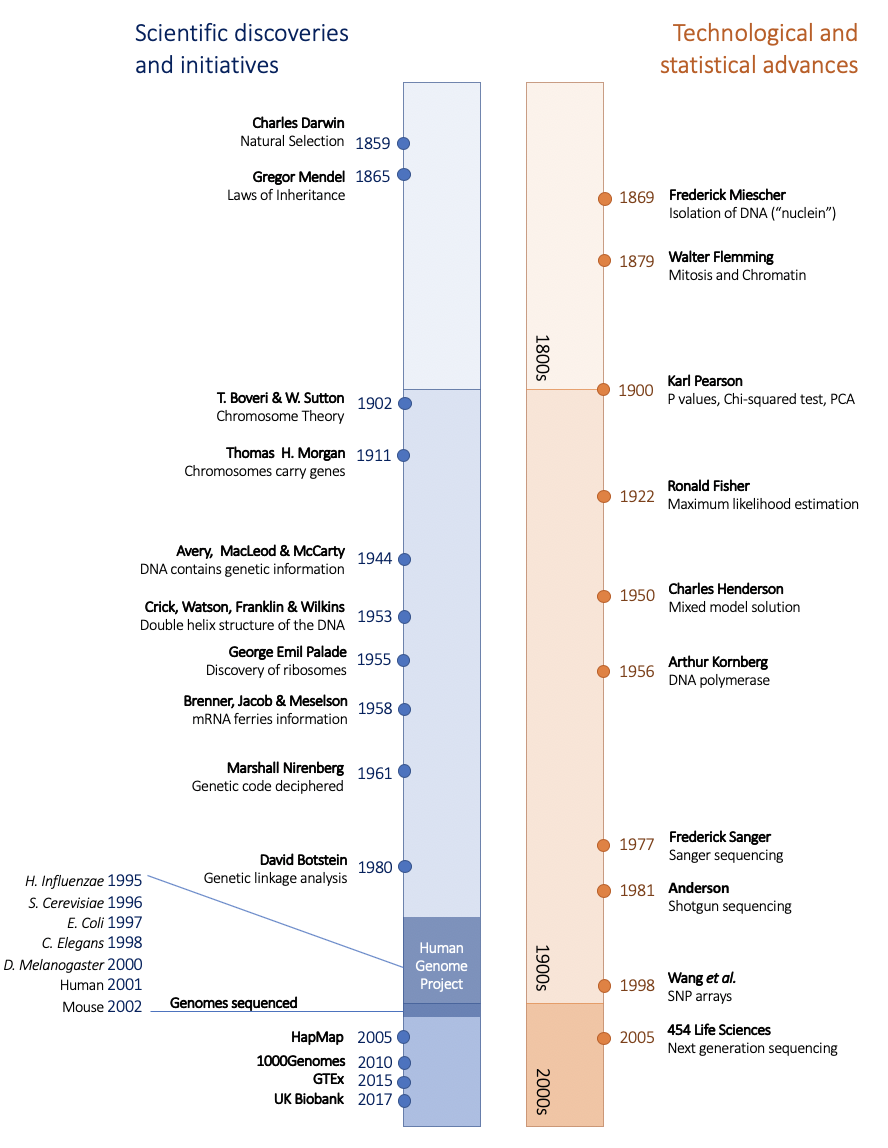
\includegraphics[width=13cm]{Chapter1/Fig/genetic_timeline_draft.png}
\caption[\textbf{Genetic Timeline}]{\textbf{Genetic Timeline (draft)}.\\
Key scientific discoveries in genetics and corresponding technological advancements.}
\label{fig:genetic_timeline}
\end{figure}

\subsubsection{Cracking the code}

Many fundamental discoveries driven by technological evolution greatly contributed to
our understanding of the function and structure of our genome and the role of genomic variation.\\

The hypothesis that there was a one-to-one correspondence between genes and enzymes was first formulated by George Beadle and Edward Tatum in 1941, based on experiments they performed on the red bread mold, \textit{Neurospora crassa}.\\

% In 1944, Barbara McClintock  discovers transposons, "jumping" genes that ... \\

In 1955, Joe Hin Tjio discovered that the human genome is comprised of exactly 46 chromosomes.
In 1955, Arthur Kornberg and colleagues isolated DNA polymerase, en enzyme that is able to copy DNA, in \textit{E. coli}.
% DNA polywhich will later be used for sequencing.\\

In 1958, Matthew Meselson and Franklin Stahl demonstrate mechanisms of DNA replication by showing that it replicates semiconservatively: each strand from the parent DNA molecule ends up paired with a new strand from the daughter generation.

% The resolution of the \gls{dna} structure and all discoveries that lead to it brought forward an understanding of other biological concepts such as protein synthesis and enabled
In the same year, Francis Crick first postulated the central dogma of biology: information is transmitted from nucleic acids (\gls{dna} and RNA) to proteins, but information cannot be transmitted from a protein to \gls{dna} \cite{crick1958protein}. 
% The deciphering of the genetic code through Nirenberg and others followed a few years later [Nirenberg \& Matthaei, 1961; Crick \& al., 1961; Matthaei \& al., 1962].\\

In the following years, Sydney Brenner, François Jacob and Matthew Meselson discover the role of mRNA in transferring information from DNA in the nucleus to the protein-making machinery in the cytoplasm (1961).\\

In 1966, Nirenberg deciphered the genetic code, discovering that combinations of three base pairs (called codons) code for 1 of 20 amino acids (fig?).
% or a stop codon (amber, ochre, opal).
\\

One major leap in understanding the biological basis of genetic variation was the development, in 1975, of \gls{dna} sequencing. 
Two different \gls{dna} sequencing techniques were independently developed by Frederick Sanger's lab and Walter Gilbert together with Allan Maxwell.\\

% Sanger’s method of \gls{dna} sequencing with chain-terminating inhibitors eventually became the standard for \gls{dna} sequencing and subsequent innovations lead to the development of automatic sequencing machines which allowed for sequencing lengths of about one kilobase. 
% For sequencing longer stretches of \gls{dna}, a novel strategy named shotgun sequencing was developed. 
% In shotgun sequencing, the long \gls{dna} of interest is randomly broken up into shorter \gls{dna} fragments which are cloned and sequenced separately. 
% The occurrence of overlapping \gls{dna} fragments given by the random nature of creating the short fragments allows for the in silico reconstruction of longer \gls{dna} fragments.

The next year the first genetic engineering company, Genentech, was founded by XX. shotgun, insulin (?)\\


1983: PCR (polymerase chain reaction) is invented 


In these same years multiple genomic features were discovered, such as transposons (1944, Barbara McClintock), introns (1977, Roberts and Sharp)


\subsubsection{Understanding disease}

In parallel, along with our understanding of the molecular structure of genes and the genome, scientists began to investigate the molecular basis of disease.

% 1902: Garrod says that alkaptonuria is mendelian


In 1956, Ingram for the first time traced the case of a disease to a genomic alteration.
He discovered that sickle cell disease, ..

% 1959: Down is caused by trisomy 21

% 1961: Screen for metabolic defect (Guthrie)

In 1980, David Botstein descibed genetic linkage studies, where ... \cite{botstein1980construction}

In 1983, the first disease gene  wasmapped.
Gusella and colleagues linked a gene on chromosome 4 to Huntington's disease. \cite{gusella1983polymorphic}

Shortly after followed a study from Francis Collins and others, identifying the genetic basis of cystic fibrosis as a single base deletion on chromosome 7 (1989)  \cite{riordan1989identification}.

% Early success in identifying genetic factors responsible for human trait and diseases, was predominantly for monogenic disorders through the use of genetic linkage studies, first proposed in 1980 \cite{botstein1980construction, botstein2003discovering}.
As of 2003, about 1,200 genes were linked to Mendelian
traits \cite{botstein2003discovering}.



candidate gene analysis (Tabor et al., 1988). \cite{tabor2002candidate}

\subsubsection{Sequencing of the first genomes}
 

In 1995, the first genome of a living organism –the bacteria \textit{H. influenzae}– was sequenced and assembled by shotgun sequencing. 
The genomes of other model organisms were to follow in subsequent years (yeast \cite{goffeau1996life}, \textit{C. elegans} \cite{c1998genome}, \textit{D. melanogaster} \cite{adams2000genome}) until the first draft of the human genome was published in 2001 \cite{lander2001initial}.

The sequence of the human genome, the development of faster, massively-parallel next-generation sequencing techniques (reviewed in [Shendure et Ji, 2008; Heather et Chain, 2016]) and \gls{dna} microarrays that allow for the genotyping of hundreds of thousands of genetic markers simultaneously [Wang et al., 1998], started a new era of human genetic and genomic research.


% \subsubsection{Genotype mapping}

\subsubsection{The Human Genome Project}

\cite{lander2001initial}

A driving force behind the growth and success of genetic association studies has been technological evolution; breakthroughs in \gls{dna} sequencing and genotyping have pushed human disease research forward, inducing a shift in the field each time technologicaladvances are introduced to the market. 
The first major breakthrough to dramatically change the landscape of genetics was the Human Genome Project (HGP), which United States President Clinton referred to as "an epic-making triumph of science and reason" (Clinton, 2000) at the announcement of its completion.\\

After the White House announcement in 2000 and a first publication in 2001, the 
project was truly completed on April 25th, 2003, on the 50th anniversary years of the Watson and Crick paper describing the helical structure of \gls{dna}.
the HGP provided the first map of the ~3 billion bases in the human genome (Lander et al., 2001; Schmutz et al., 2004; Hattori, 2005). 
The HGP was a massive international undertaking and a truly collaborative effort; sequencing and analysis took place across twenty centers in six different countries (USA, UK, France, Germany, Japan, China) and took 13 years to complete, costing approximately \$2.7 billion (National Human Genome Research Institute, 2003b).\\ 

Additional breakthroughs in sequencing technologies have expanded and refined the reference genome, which now captures more than 92\% of the genome and provides a landscape of its 20,000 genes \cite{lander2001initial}.\\

With a complete map of the human genome in place, it was now easy to identify genetic variants, those bases discovered in an individual that did not match the (reference) base annotated in the map of the human genome. 
More common (\gls{maf} >5\%) variants were called single nucleotide polymorphisms (SNPs). 
Previous studies had estimated that approximately 0.1\% (1 base per 1,000) of an individual's genome was a polymorphism (Li and Sadler, 1991; Wang, 1998; Cargill et al., 1999). 
Most of these polymorphisms were scattered across the genome and no one had yet broadly described what these variants were, where in the genome they resided, and what (if any) phenotypic effect they conferred.\\

The International HapMap Project was the first effort of its kind to systematically catalogue such variation. 
It was officially started in October 2002 as a collaboration between research groups and provate companies in Canada, China, Japan, Nigeria, the United Kingdom and the United States with the aim to develop a haplotype map (HapMap) of the human genome \cite{international2003international}.
By genotyping individuals of African (YRI), European (CEU) and East Asian (JPT, CHB) descent, HapMap assembled Phase I (2005) of a publicly available database of common variants (>5\% \gls{maf}) in global samples \cite{international2005haplotype}. 
The HapMap expanded rapidly. 
By Phase II (2007), the database contained 2.1 million SNPs from the four original populations (Frazer et al., 2007) \cite{international2007second}.
Phase III (2010) added genotyping from seven additional populations, for a total of >3 million SNPs in 11 global ancestry groups \footnote{ASW (African ancestry in Southwest USA); CEU (Utah residents with Northern and Western European ancestry from the CEPH collection); CHB (Han Chinese in Beijing, China); CHD (Chinese in Metropolitan Denver, Colorado); GIH (Gujarati Indians in Houston, Texas); JPT (Japanese in Tokyo, Japan); LWK (Luhya in Webuye, Kenya); MEX (Mexican ancestry in Los Angeles, California); MKK (Maasai in Kinyawa, Kenya); TSI (Tuscans in Italy); YRI (Yoruba in Ibadan, Nigeria).} (Altshuler et al., 2010).\\ 
With the map of the genome complete and cataloguing efforts moving apace, researchers could now begin to search for modest effect genetic variants associated to human disease across the full length of the genome.

% \subsection{The International HapMap Project}

% Aim:  \cite{international2003international}.
% Officially started in 2002 as a collaboration between research groups and provate companies in Canada, China, Japan, Nigeria, the United Kingdom and the United States.\\

% phaseI: 2005 \cite{international2005haplotype}
% phaseII: 2007 \cite{international2007second}
% phaseIII: 2009

% Four populations: 
% \begin{itemize}
%     \item 30 Yoruba trios from Ibadan, Nigeria (YRI)
%     \item 30 trios of Utah residents of northern and western European ancestry (CEU)
%     \item 44 unrelated Japanese individuals from Tokyo, Japan (JPT)
%     \item 45 unrelated Han Chinese individuals from Bejing, China (CHB)
% \end{itemize}

% In phase III, 11 global ancestry groups have been assembled: ASW (African ancestry in Southwest USA); CEU (Utah residents with Northern and Western European ancestry from the CEPH collection); CHB (Han Chinese in Beijing, China); CHD (Chinese in Metropolitan Denver, Colorado); GIH (Gujarati Indians in Houston, Texas); JPT (Japanese in Tokyo, Japan); LWK (Luhya in Webuye, Kenya); MEX (Mexican ancestry in Los Angeles, California); MKK (Maasai in Kinyawa, Kenya); TSI (Tuscans in Italy); YRI (Yoruba in Ibadan, Nigeria).

% %********************************** % 1.1.1  **************************************
\subsection{Genome-wide association studies}

The data generated by the International HapMap Project combined with development of appropriate chip-based microarray technology, enabling simultaneous genotyping of more than one million SNPs, led to the first wave of genome-wide association studies (GWAS).

Briefly, GWAS are a hypothesis free approach to test for significant association between the genotype frequency of common genetic variants (one by one across the entire genome) and a trait of interest \cite{mccarthy2008genome}. 

The first successful GWAS conducted in 2005 for age-related macular degeneration (AMD) using 96 cases and 50 healthy controls, tested for associations at ~100,000 SNPs \cite{klein2005complement}. 



In 2007, the Wellcome Trust Case-Control Consortium (WTCCC) published a study where they performed GWAS on seven different common diseases, using a common set of 3,000 healthy controls and 2,000 cases for each of bipolar disorder (BD), coronary artery disease (CAD), Crohn's disease (CD), hypertension (HT), rheumatoid arthritis (RA), type I and II diabetes (T1D, T2D), \cite{wellcome2007genome}.\\ 

In 2008, the GWAS Catalog was founded to keep a record of all published GWAS and identified associations \cite{}.

\cite{welter2014nhgri}

As of June 4th, 2020, the GWAS Catalog includes 4,566 publications, describing 186,829 associations between 124,935 genetic variants and XX traits or diseases.



% \subsection{GWAS Catalog}

% GWAS Catalog was founded by \gls{nhgri} in 2008
% and has become a collaborative project between the \gls{nhgri} and the \gls{ebi} since 2010
% GWAS Catalog publications: https://www.ebi.ac.uk/gwas/docs/related-resources\\

% GWAS Catalog Stats:
% Last data release on 2020-06-04
% 4,566 publications
% 124,935 SNPs
% 186,829 associations

% \subsection{The 1000 Genomes Project}

% The 1000 Genomes Project ran between 2008 and 2015, creating the largest public catalogue of human variation and genotype data.
% The final data set contains data for 2,504 individuals from 26 populations\\

% pilot: 2010 \cite{10002010map}
% phase 1: 2012 \cite{10002012integrated}
% phase 3: 2015 \cite{10002015global, sudmant2015integrated}\\


% Whilst these early GWAS were based on the directly genotyped tag SNPs, from 2008 onwards, utilisation of methods to fill in missing genotype data became increasingly common practice, referred to as imputation (ref). 

% Imputation is a statistical technique to infer genotypes. 
% The general idea is to compare genotyped samples to a reference panel of individuals of similar ancestry to identify short haplotype stretches that are shared between the genotyped and reference samples (Fig. 1.3b). This then allows missing genotypes to be filled in.
% Initially, data from the HapMap Project was used as a reference panel, with for example the CEU panel used to impute samples of European ancestry. 
% Imputation is now also used to explore association effects of rare variants (see Section 1.2.1 for further details of imputation of rare variants, including examples of current reference panels used).

% Initially, GWAS focused on complex phenotypes with binary outcomes, using a case control design. 
% For each SNP and binary trait, the association was therefore often evaluated using a Cochran–Armitage (trend) test
% $\chi^2$ test or a Fisher's exact test comparing the numbers of cases and controls when stratified by their allelels at the locus of interest.

% Quantitative traits have since become increasingly popular to use as phenotypes. 
% % This is partly due to the fact that the onset of many diseases is time dependent, meaning that some individuals selected as controls may later become cases and hence the control group actually contains a mixture of cases and controls, resulting in some loss of power. 
% % In addition, some binary traits are defined by thresholding a continuous variable, with the threshold somewhat arbitrary such that an individual with a value marginally greater than the cutoff is said to be `diseased' whilst an individual just below the threshold is defined as `healthy'.
% % Examples include defining obesity based on a BMI threshold and diabetes based on fasting glucose levels. 
% % This thresholding approach results in loss of information regarding phenotypic similarity and as a result, using the binary outcome is likely to be less powered than using the underlying quantitative trait. 
% % Moreover, quantitative traits are often closer to the underlying biology, providing greater insight into the mechanisms underpinning trait or disease development and the results from using continuous traits may be more directly interpretable, in that it is possible to quantify the average difference in trait outcome per risk allele carried.

% Furthermore, linear regressions and their derivations have become more popular methods to assess association, due to their flexibility to include covariates \cite{mccarthy2008genome}.
% I describe these models in detail in the next Chapter (Chapter 2). 

% As of 2020 when I am writing this thesis, over 70,000 associations have been identified for over 1,000 different traits and diseases, according to the GWAS Catalog (ref).

% Linkage disequilibrium (LD, The nonrandom allocation of alleles at nearby variants to individual chromosomes as a result of recent mutation, genetic drift or selection, manifest as correlations between genotypes at closely linked markers.)

% Hardy-Weinberg equilibrium (HWE,A theoretical description of the relationship between genotype and allele frequencies that is based on expectation in a stable population undergoing random mating in the absence of selection, new mutations and gene flow: in the context of genetic studies, departures from equilibrium can be used to highlight genotyping errors).

% \cite{mccarthy2008genome}

\gls{gwas} results are often visualised using Manhattan plots, with the negative log p value plotted on the y-axis against the corresponding genomic position ordered by chromosome and position on the x-axis. 
Peaks on these plots represent loci (multiple variants in \gls{ld}) that display evidence of association with the analysed phenotype. 
Variants are deemed to be significantly associated with a trait if they exceed an appropriately chosen p value threshold. 
Due to \gls{ld} structure, if a peak arises from a single variant, this is usually indicative of a false positive finding.

\begin{figure}[h]
\centering
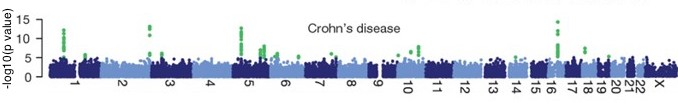
\includegraphics[width=15cm]{Chapter1/Fig/Manhattan_plots_CD_WTCCC_2007.jpg}
\caption[\textbf{Manhattan plot}]{\textbf{Manhattan plot}.\\
Manhattan plot for Crohn's disease (CD) from the WTCCC study \cite{wellcome2007genome}}
\label{fig:molecular_genetic_associations}
\end{figure}

\subsubsection{From case-control to cohort studies}

UK Biobank ~ 500,000 individuals \cite{bycroft2018uk}



Reviews:

Goals of GWAS (2005) \cite{hirschhorn2005genome}

5 years of GWAS (2012) \cite{visscher2012five}

10 years of GWAS (2017) \cite{visscher201710}

\subsubsection{Challenges in GWAS}

% Rare diseases: often rare variants too (\gls{maf}<0.05)
% Pleiotropy: same variant affects multiple traits

% non-additive interactions:
% Epistasis: combined effect of separate variants interacting to have an effect on trait
% GxE:interaction between a variant and an environment


% \subsection{Genotype-Environment interactions}

% Explicitly, whilst a variant with a significant genetic effect is determined by a mean phenotypic difference between groups of individuals with different allele dosages and a significant environment effect is determined by a mean phenotypic shift that is constant across different allele dosages (Fig. 1.6b), a significant statistical interaction effect is defined when there is a significant difference in the genetic effect between two groups of individuals with different environmental exposures.

% % \begin{figure}[h]
% % \centering
% % 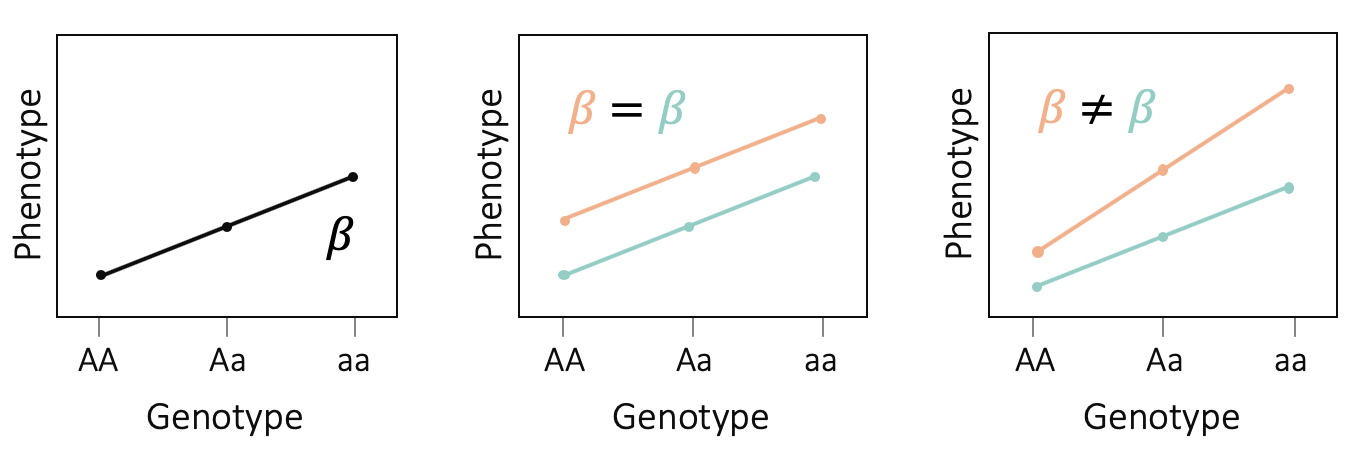
\includegraphics[width=15cm]{Chapter1/Fig/GxE.png}
% % \caption{\textbf{Illustration of GxE effect}.\\
% % a) Genetic effects only. b) Environments have effects on phenotype but do not change the genetic effect. c) Interaction effect between genotype and environment (GxE).}
% % \end{figure}

% \newpage

% %********************************** %Second Section  **************************************
% \section{Gene expression and eQTL mapping}  %Section - 1.2 

% Intro on molecular readouts as intermediate to understand genotype-phenotype mechanisms.
% Going back in time to our progressive better understanding of moelcular machinery, starting from Crick postulating the central dogma.

% % \subsection{\gls{dna} and the central dogma}
% \subsection{Gene regulation}

% The resolution of the \gls{dna} structure and all discoveries that lead to it brought forward an understanding of other biological concepts such as protein synthesis and enabled Francis Crick to postulate the central dogma of biology: information is transmitted from nucleic acids (\gls{dna} and RNA) to proteins, but information cannot be transmitted from a protein to \gls{dna} \cite{crick1958protein}. 
% The deciphering of the genetic code through Nirenberg and others followed a few years later [Nirenberg \& Matthaei, 1961; Crick \& al., 1961; Matthaei \& al., 1962].\\

% Today, we know that \gls{dna} gets transcribed into RNA aided by the \gls{dna} polymerase molecule, and RNA gets translated to amino-acids making up proteins in the ribosome, with the help of transfer RNA (tRNA).\\

% In the process of gene expression, the genetic information stored in the \gls{dna} is used to produce molecular products. 
% The information on the composition of these products is contained in restricted portions of the genome known as genes. 
% In the first step of gene-expression (transcription), genes are transcribed into ribonucleic acid (RNA) molecules. 

% Although RNA molecules can be the final product of gene expression, many RNA molecules are translated into proteins in a process known as translation. 
% Proteins are long chains of smaller molecules called amino acids. 
% Only approximately 1.5\% of the human genome codes for proteins (Lander et al., 2001) while a large fraction of the remaining portion is likely to play a role in the regulation of gene expression (ENCODE Project Consortium, 2004). 

% The impact of genetic variation on phenotypes is the consequence of perturbations to this complex molecular machinery.
% An easily interpretable mechanism through which genetic variants may affect phenotype is the direct alteration of the structure of the coded protein and thus of its functionality. 
% For example, sickle cell anaemia is caused by a \gls{snp} in the \textit{HBB} gene, which causes a substitution of an amino acid in the sequence of the coded protein (Laird and Lange, 2010). 
% Alternatively, genetic variation may affect the regulation of gene expression. 
% One way this can occur is through the disruption of a specific sequence that affects the binding of proteins regulating the expression of a gene, for example a transcription factor (TF). 
% Another possibility is the alteration of the structure of the \gls{dna}, thereby affecting the functionality of regulatory elements and ultimately gene expression (ENCODE Project Consortium, 2004; Kundaje et al., 2015). 

% \subsection{Estimation of gene expression levels}



% In this thesis, we focus on gene expression, i.e., the transcriptome, as a molecular phenotype.
% In general, the transcriptome describes the complete set of transcripts in a tissue or cellular sample, and their respective quantity. 
% As a precursor of protein expression, mRNA can serve as a proxy of gene expression levels. 
% Multiple approaches have been developed to measure cellular mRNA levels, including hybridization- and sequencing-based approaches. 
% In the case of hybridization-based methodology, reverse transcription (RT) is used to generate a complementary \gls{dna} (c\gls{dna}) template of the mRNA. 
% When this c\gls{dna} template is being amplified with labelled hybridization probes via quantitative polymerase chain reaction (qPCR), fluorescence is emitted according to the oligonucleotides that are being incorporated. 
% Based on the fluorescence signal, the genetic sequence of the original mRNA strand can be reconstructed. 
% Alternatively, a hybridization microarray contains pre-defined probes for transcripts of every known gene of one or several species. Transcripts that are not known a priori can be detected with tag-based methods such as SAGE (Serial Analysis of Gene Expression); SAGE uses small tags that cover only fragments of a transcript as probes, and can therefore, opposed to hybridization microarray chips, also discover transcripts whose full sequence is unknown. 
% However, a large proportion of the tags used by SAGE does not map to unique regions of a reference genome due to their short length, and can therefore not be used for transcript quantification. 
% Further, tag-based approaches do not ensure the analysis of the entire transcriptome, and can generally not discover alternative splicing events (Wang et al., 2009).
% RNA sequencing (RNA-Seq) based on next-generation sequencing (NGS) of the c\gls{dna} allows for genome-wide quantification of the transcriptome. After obtaining one (single-read RNA-Seq) or two paired (paired-end RNA-Seq) sequence reads per c\gls{dna} fragment, the sequencing reads are either aligned to a reference genome or are assembled de novo. 
% From the number of RNASeq reads that map to a particular gene an estimation of gene expression can be deduced. 
% In this thesis, we use FPKM (fragments per kilo base per million reads mapped) for gene expression estimations. 
% FPKM quantify the number of reads that are assigned to a given gene, normalised by gene length and the total sequencing depth (Wang et al., 2009).
% Opposed to the hybridization- and tag-based methods, NGS allows for identifying completely new genes, previously unknown genetic variants in the genes, variation in alternative splicing, or post-transcriptional modifications. In addition, RNA-Seq can quantify the vast array of non-coding RNA molecules (Section 1.1.1). Altogether, sequencing-based assessments of the transcriptome deliver more detailed insights into gene expression variability than hybridization- or tag-based approaches.
% In this thesis, we quantify gene expression by RNA-Seq measurements of mRNA levels.

% The human genome project revealed that human \gls{dna}
% consists of surprisingly few exons (1.1\% of the genome), whereas introns cover 24\% of the genome (Venter et al., 2001; Lander et al., 2001). 
% The number of genes was also found to be smaller than expected, with around 30,000 being identified in 2001, and 19,000 genes being the latest estimate at the time that this thesis is written (Ezkurdia et al., 2014). 

% \subsubsection{From microarrays to (bulk) RNA-sequencing}



% Useful for comparative transcriptomics, e.g. samples of the same tissue from different species.
% Useful for quantifying expression signatures from ensembles, e.g. in disease studies.
% Insufficient for studying heterogeneous systems, e.g. early development studies, complex tissues (brain)
% Does not provide insights into the stochastic nature of gene expression

\begin{figure}[h]
\centering
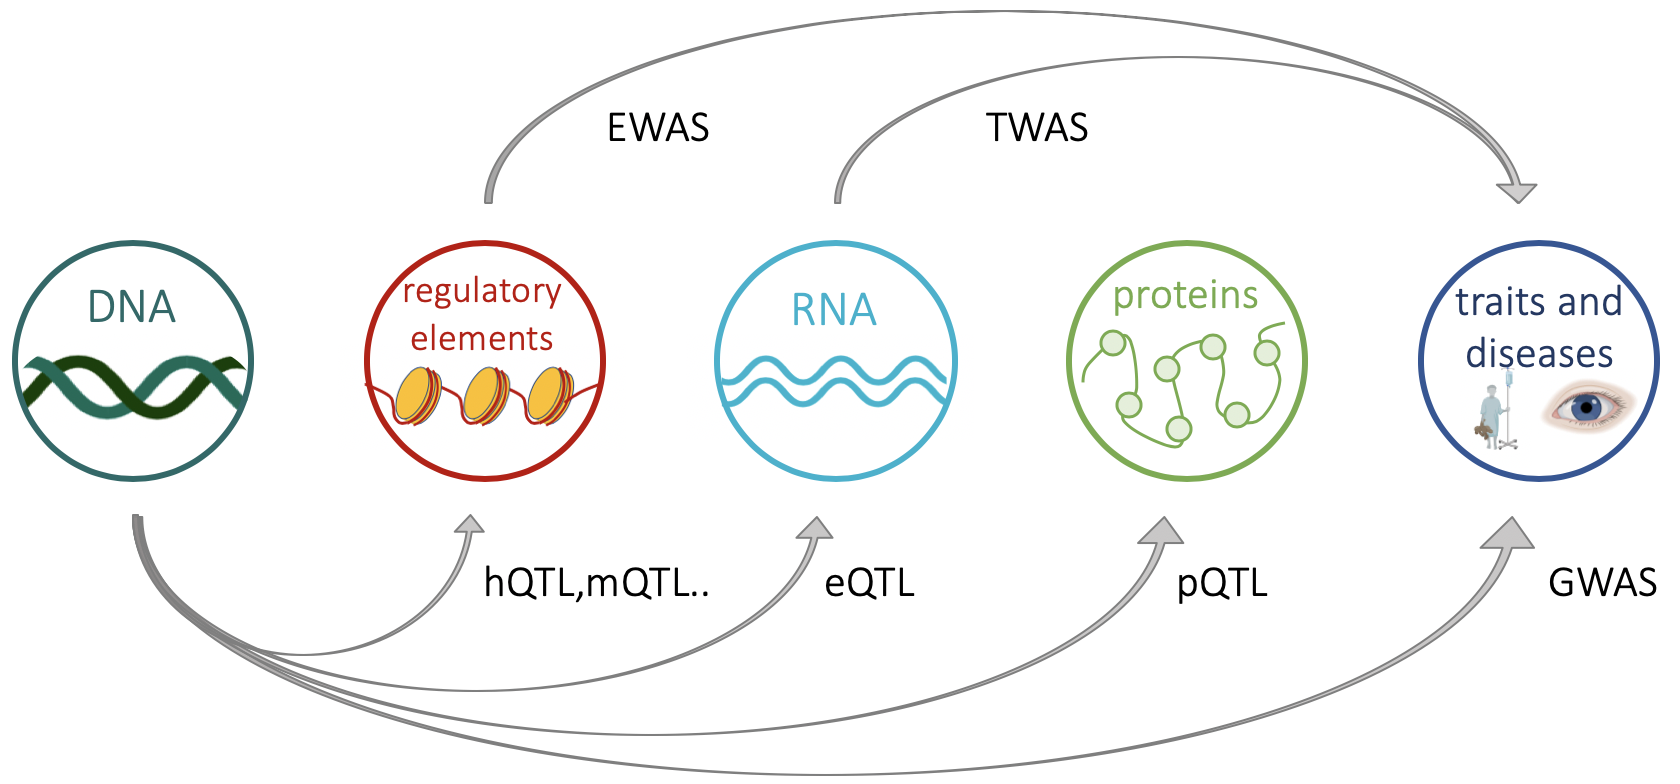
\includegraphics[width=15cm]{Chapter1/Fig/layers_of_genetic_associations_draft.png}
\caption[\textbf{Genetics of molecular and global traits}]{\textbf{Genetics of molecular and global traits}.\\
Layers of genetic association analyses to understand the molecular mechanisms underpinning the genotype-phenotype map}
\label{fig:molecular_genetic_associations}
\end{figure}

% %********************************** % 1.1.8  **************************************
\subsection{Expression quantitative trait loci}\label{sec:eqtl}

first eqtl using microarray in yeast 2002 \cite{brem2002genetic}\\

\textbf{first eqtl map in mammals 2003}
The decrease in cost of high-throughput profiling of gene expression has made it possible to measure gene expression levels in large numbers of individuals, thereby enabling the mapping of quantitative trait loci for gene expression (eQTL mapping, Schadt et al., 2003). \cite{schadt2003genetics}

review: rockman and kruglyak 2006 \cite{rockman2006genetics}\\

Bulk RNA-sequencing was a major breakthrough in the late 2,000s (ref) and has been widely used since.
It measures the average expression level for each gene across a large population (N=) of input cells. 
First eqtl mapping using RNA-seq: 2010
\cite{montgomery2010transcriptome, pickrell2010understanding}

review: 2014 \cite{westra2014genome}\\

\textbf{GTEx}:
As genetic effects on molecular traits may depend on factors such as tissue, environment and cell type, it is necessary to measure expression and other molecular traits in disparate cellular contexts. 
For this reason, the Genotype-Tissue Expression Project (GTEx has been collecting and analysing gene expression profiles across several primary tissues collected from post-mortem donors.
Since the publication of their pilost study in 2015 \cite{gtex2015genotype}, several versions have been published \cite{gtex2017genetic, aguet2019gtex}.
Version 8 was released in 2019 and it includes data from 53 tissue types\footnote{Adipose - Subcutaneous, Adipose - Visceral (Omentum), Adrenal Gland, Artery - Aorta, Artery - Coronary, Artery - Tibial, 
Brain - Amygdala, Brain - Anterior cingulate cortex (BA24), Brain - Caudate (basal ganglia), Brain - Cerebellar Hemisphere, Brain - Cerebellum, Brain - Cortex, Brain - Frontal Cortex (BA9), Brain - Hippocampus, Brain - Hypothalamus, Brain - Nucleus accumbens (basal ganglia), Brain - Putamen (basal ganglia), Brain - Spinal cord (cervical c-1), Brain - Substantia Nigra, 
Breast - Mammary Tissue, Cells - Cultured fibroblasts, Cells - EBV-transfortmed lymphocytes,  Cervix - Ectocervix, Cervix - Endocervix, Colon - Sigmoid, Colon - Transverse, Esophagus - Gastroesophageal Junction, Esophagus - Mucosa, Esophagus - Muscularis, Fallopian Tube, Heart - Atrial Appendage, Heart - Left Ventricle, Kidney - Cortex, Kidney - Medulla, Liver, Lung,  Minor Salivary Gland, Muscle - Skeletal, Nerve - Tibial, Ovary, Pancreas, Pituitary, Prostate,  Skin - Not Sun Exposed (Suprapubic), Skin - Sun Exposed (Lower leg), Small Intestine - Terminal Ileum, Spleen, Stomach, Testis, Thyroid, Uterus, Vagina, Whole Blood} from 948 donors.

% Other such as splicing, trans?



% In addition, eQTL have been described in iPSC (dicussed later in Section 4)
% % add box on overview of tissues with available eQTL

% \subsection{Interpreting eQTL}

% colocalization

% \newpage

%********************************** %Third Section  **************************************
% \section{Single cell RNA-seq}  %Section - 1.3 

% Next generation sequencing approaches have been applied to individual cells to quantify variation in \gls{dna} sequence, mRNA expression, epigenetic marks and protein abundance at single cell resolution.
% In this thesis, we focus on transcriptomic assays, which encompass the large majority of single-cell genomic research published to date (ref). 
% I use this section to provide an introduction to \gls{scrnaseq}.
% First, I summarise the processes involved in generating single-cell expression data and describe the technologies.. (1.3.1)
% Next, I provide an overview of computational modelling to analyse scRNAseq data (1.3.2).
% Finally, I identify examples in areas of biology where these assays have provided insight (1.3.3).


% \subsection{Evolution of scRNA-seq technologies}

% % from the tutorial (martin hemberg, davis - resource in the HCA)
% scRNA-seq was first introduced in 2009 by Tang \textit{et al.} \cite{tang2009mrna}
% Did not gain widespread popularity until ~2014 when new protocols and lower sequencing costs made it more accessible.

% Currently there are several different protocols in use, e.g. SMART-seq2 \cite{picelli2013smart}, CELL-seq \cite{hashimshony2012cel} and Drop-seq \cite{macosko2015highly}.

% There are also commercial platforms available, including the Fluidigm C1, Wafergen ICELL8 and the 10X Genomics Chromium.

% The first single-cell RNA sequencing (scRNA-seq) experiment was published in 2009, and the authors profiled only eight cells \cite{tang2009mrna}. 
% Only 7 years later, 10X Genomics released a data set of more than 1.3 million cells (ref).

% The main difference between bulk and single cell RNA-seq is that each sequencing library represents a single cell, instead of a population of cells. 
% Therefore, significant attention has to be paid to comparison of the results from different cells (sequencing libraries). 
% The main sources of discrepancy between the libraries are:

%  - Amplification (up to 1 million fold)
%  - Gene ‘dropouts’ in which a gene is observed at a moderate expression level in one cell but is not detected in another cell (Kharchenko, Silberstein, and Scadden 2014).
% In both cases the discrepancies are introduced due to low starting amounts of transcripts since the RNA comes from one cell only. 
% Improving the transcript capture efficiency and reducing the amplification bias are currently active areas of research. 
% However, as we shall see in this course, it is possible to alleviate some of these issues through proper normalization and corrections.

% \begin{itemize}
%     \item CEL-seq (cell expression by linear amplification and sequencing) \cite{hashimshony2012cel}
%     \item CEL-seq2 - Hashimshony et al 2016
%     \item Drop-seq \cite{macosko2015highly}
%     \item InDrop-seq \cite{klein2015droplet}
%     \item MARS-seq (massively parallel single cell RNA-seq) \cite{jaitin2014massively}
%     \item SCRB-seq - Soumillon et al 2014
%     \item Seq-well \cite{gierahn2017seq}
%     \item SmartSeq \cite{ramskold2012full}
%     \item SmartSeq2 \cite{picelli2013smart}
%     \item SmartSeq3 \cite{hagemann2020single}
%     \item STRT-seq \cite{islam2011characterization}
% \end{itemize}



% The methods can be categorised in different ways, but two of the most important aspects are quantification and capture

% Quantification: full-length vs tag-based\\

% Capture: microwell- (or plate-), microfluidic-, droplet-based.\\



% % make figure plate vs droplet based scRNA-seq

% Quantifying gene expression via microscopy is familiar in contemporary biology, whether using hybridisation techniques or artificially-created fluorescent fusion proteins. 
% The amount of fluoresence that is observed in individual cells directly provides the readout of RNA or protein expression levels. 
% Flow cytometry scales up these optical approaches to hundreds of thousands of measurements without compromising cellular resolution [12]. 
% Historically, these methods have not been suitable for assaying many genes simultaneously, due to constraints imposed by fluorophore emission and absorption spectra. 
% Nucleotide-focussed methods pushed beyond this limitation: real time polymerase chain reaction (PCR) [13] can quantify hundreds of genes, with cellular throughput improved using microfluidic systems [14, 15].
% The recent development of sequencing-by-hybridisation (described in Section 1.4.5) provides an interesting combination of these two approaches, allowing the precise localisation and quantification of thousands of transcripts per-cell.\\

% To achieve truly transcriptome-wide expression coverage, however, RNA-seq based methods are best suited. 
% Shortly after the first application of RNA-seq to bulk populations of cells [16], the feasibility of applying RNA-seq to individual cells was demonstrated [7]. 
% Over the past five years, single-cell RNA-sequencing (scRNA-seq) has become the most commonly used approach for assaying single-cell gene expression profiles. 
% There are two broad sets of methods for applying single-cell RNA-seq—“plate-based” and “droplet-based” (Figure 1.1).\\

% Initially, most studies used plate-based assays, where library preparation is performed manually on cells sorted into and lysed in individual wells of a microwell plate (Figure 1.1) [17, 18].
% Robotic and microfluidic systems (e.g., Fluidigm C1) have been developed to automate some of these processes.\\

% Droplet-based methods employ microfluidics to capture individual cells in nanolitre sized droplets, each loaded with reagents and unique labels: reverse transcription and transcript labelling take place within these small volumes (Figure 1.1). 
% The droplet suspension is later broken down for pooling of cell libraries prior to sequencing. 
% These methods have been developed by academic groups [19, 20] and commercially, by 10X Genomics [21].\\

% Each approach has its own advantages and disadvantages. 
% Plate-based methods tend to provide higher-quality libraries at the cost of lower cellular throughput, processing hundreds or thousands of cells compared to the hundreds of thousands that droplet methods can achieve.

% More subtle differences also differentiate the two sets of methods. 
% To capture rare cell types with known cell-surface markers, it is generally more efficient to flow-sort and prepare plates of single-cell libraries rather than the brute-force approach of capturing more cells outright using a droplet method. 
% Additionally, current droplet methods capture gene information exclusively from the 3’ or 5’ end of each transcript, while some plate approaches generatereads from across entire transcripts; the latter allows splice-variant and allele-specific transcriptional information to be retrieved. 
% Finally, droplet methods are more likely to produce “multiplet" cell transcriptomes, where multiple different cells become labelled with the same barcode. 
% This is largely due to the lack of user oversight (e.g., it is more difficult to identify attached pairs of cells) and the possible reuse of cell barcodes from the labelling beads. 
% The doublet rate in droplet experiments is proportional to the number of loaded cells [21]; hence a user may reduce the rate of this confounding, albeit by sacrificing cost-efficiency, by loading fewer cells per sample.

% \begin{figure}[h]
% \centering
% 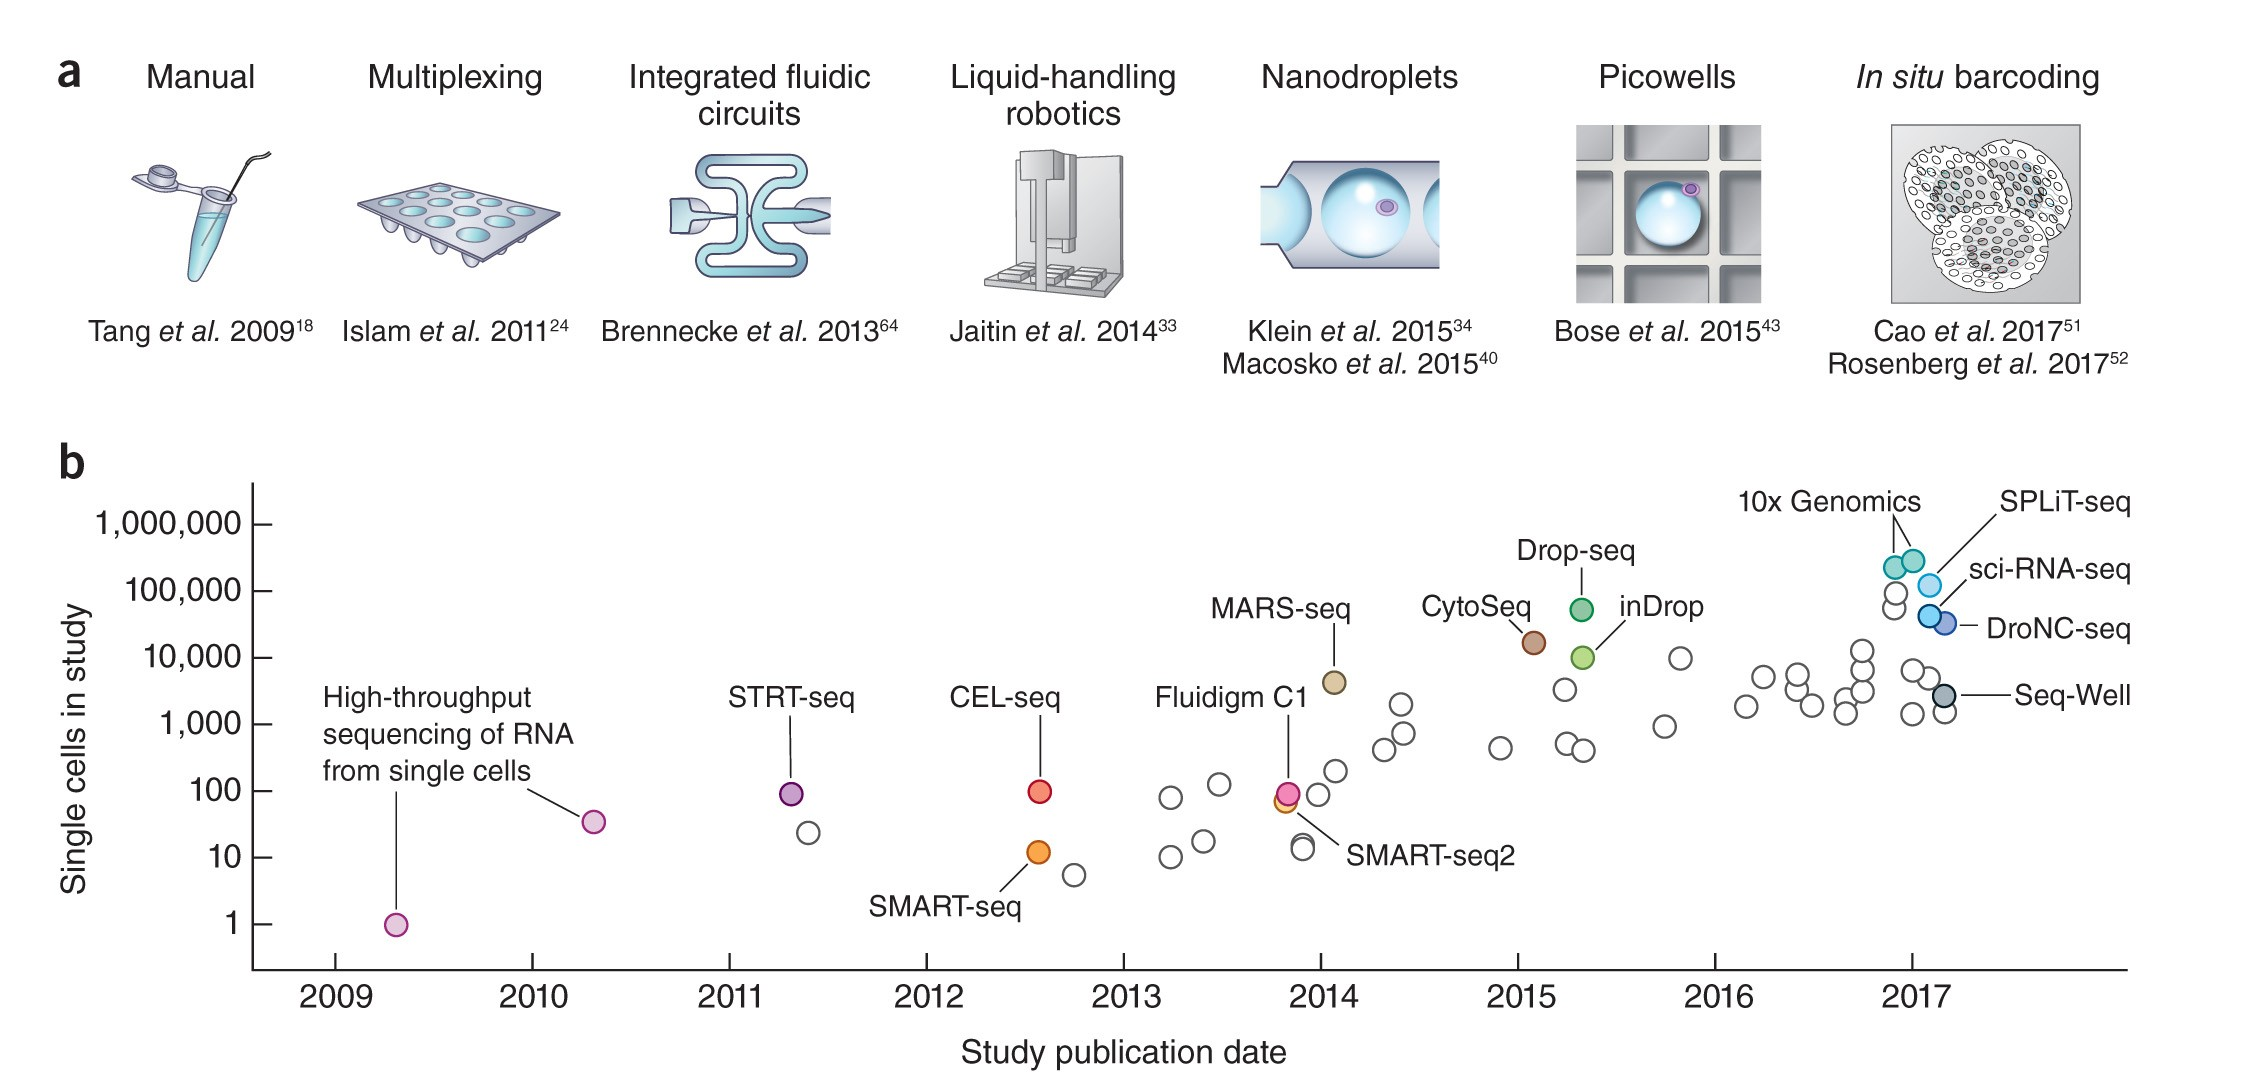
\includegraphics[width=15cm]{Chapter1/Fig/scrnaseq_technologies_svensson2018.jpg}
% \caption[\textbf{scRNA-seq technologies}]{\textbf{Scale of scRNA-seq experiments}.\\
% Technologies that have allowed....

% % make own version adding SmartSeq3 etc 

% adapted from \cite{svensson2018exponential}}
% \label{fig:scrnaseq_technologies}
% \end{figure}

% \subsubsection{Plate-based technologies}

% SmartSeq2

% \subsubsection{Droplet-based technologies}

% DropSeq, 10X Genomics

% \subsubsection{other technologies}

% multi omics aproaches (\cite{stuart2019integrative})

% spatial transcriptomics

% perturb seq

% %\subsection{Analysis of scRNA-seq data}

% \subsection{Computational modelling of scRNA-seq}

% Analysis of scRNA-seq data requires a new set of considerations, largely concerning technical signals, that were not relevant for bulk RNA-sequencing work. 
% Moreover, the resolution of this single-cell data also allows a number of more powerful analysis techniques to be applied.
% This section describes, in brief, how a typical single-cell RNA-sequencing dataset may be analysed.

% \cite{stegle2015computational}

% \subsubsection{Low-level analysis}

% reads QC 

% alignment

% mapping QC

% \subsubsection{Normalization and batch correction}

% Count matrix
% 10 Genomics: UMI counts
% Smasrtseq2: expected counts or TPM (similar to bulk)

% cell QC (e.g. remove cells with less than xx total counts, yy total genes)
% possibly deal with doublets etc - in our case, donor assignment is also here

% normalization (account for differences due to read coverage etc)

% log transformation (variance stabilising)

% \textbf{feature selection} (isolate most informative genes, e.g. highly variable genes - HVGs)\\

% genes that behave differently from your expected mean-variance relationship

% optional: centering+scaling - standardizing

% batch correction (stronger than normalisation) 
% mutual nearest neighbours (MNN, \cite{haghverdi2018batch}) - and then fastMNN
% canonical correlation analysis (CCA, implemented in Seurat \cite{butler2018integrating}), Stuart et al 2019
% LIGER iNMF (negative matrix factorization),
% Harmony (\cite{nowotschin2019emergent}) - iterative soft k means (fastest)
% Welch et al 2019, Korsunsky et al 2019


% \subsubsection{Computational analysis}

% \textbf{dimensionality reduction}

% \gls{pca} was first introduced by Pearson over a hundreds years ago (\cite{}, see section 1), yet remains one of the most widely used tools \\

% \textbf{clustering}

% unsupervised\\

% \textbf{pseudotime}

% PCA, diffusion maps\\

% \textbf{DE}

% DESeq, edgeR



% \subsubsection{Visualization techniques}

% Even after application of a dimension-reduction procedure, a typical dataset will retain more than three biologically important dimensions in its new subspace, which makes visual representation of the data challenging. 

% Transforming high-dimensional data into a human-readable format is therefore an important challenge for single-cell data interpretation.

% scRNA-seq data visualization techniques used in this thesis: 



% \begin{itemize}
%     \item \gls{pca}
%     \item t-distributed stochastic neighbour embedding (tSNE) \cite{maaten2008visualizing}
%     \item uniform manifold approximation and projection (UMAP) \cite{mcinnes2018umap}
% \end{itemize}


% Workflow packages:

% \begin{itemize}
%     \item scanpy
%     \item scater / scran / Single cell experiment (SCE)
%     \item seurat
%     \item SINCERA
% \end{itemize}




% \subsection{General applications of scRNA-seq in biology}

% Studies of single-cell transcriptomes allow us to directly investigate properties of individual cells, i.e. mRNA abundance. 
% Thus gene regulation is analyzed at the single cell level and, unlike traditional bulk RNA- sequencing, cell-to-cell heterogeneity can be considered.

% By measuring gene expression in development, differentiation, or other responses, we can start to understand cellular phenotypes as well as the regulatory processes that determine these phenotypes. 
% In many experiments cells are sampled at many time points and gene expression is assessed.

 


% \subsubsection{Atlases}

% Human Cell Atlas (HCA)

% The human cell atlas aims to provide a comprehensive reference map of all human cells
% \cite{rozenblatt2017human}
% \subsubsection{Cancer}
% \subsubsection{Immunology}
% \subsubsection{Development}

% developmental trajectories 
% A particular advantage of single-cell methods is the ability to capture cells at various developmental
% stages in a single experiment.

% \subsubsection{lineage tracing}

\newpage

\vspace*{10px}

\textit{“It is not birth, marriage, or death, but gastrulation which is truly the most important time in your life.”}\\
\rightline{Lewis Wolpert, 1986}

\vspace*{5px}

%********************************** %Fourth Section  **************************************
% \section{Human induced pluripotent stem cells}  %Section - 1.4 
\section{Human iPSCs to study cell differentiation}  %Section - 1.4 

Human induced pluripotent stem cells (iPSCs) and cells derived from them are the biological system I use throughout this thesis to study the effect of common genetic variants on expression along cell differentiation.

In this section I provide some rudiments of human embryology and describe the role of human stem cells in scientific research, focusing especially on the iPSC technology which allows us to reprogramme somatic cells to regain stem-cell like pluripotent properties and to be subsequently differentiated into virtually any desired cell type, provided the right stimuli.\\

I begin by providing a brief historical overview of the study of early development in humans and describe the key stages of human embryology.
Then, I introduce the concepts of embryonic stem (ES) cells and somatic nuclear cloning.
Next, I describe induced pluripotent stem cells, the technology behind the reprogramming and re-differentiating of iPSCs.
Finally I describe general applications of human stem cells in biology, focusing in particular on applications of iPSCs in human genetics.

% %********************************** % 1.2.1  **************************************
\subsection{From homunculi to modern embryology}

In the previous chapter, we learnt that DNA encodes all instructions of life, and that each one of us contains a mixture of genetic information from both parents, which is identically copied in every one of our cells.
But how do we go from one single cell containing our genetic fingerprint to a whole organism made of some 37 trillion highly specialised cells which differ in function and morphology and work together to ...?\\

Interest in the study of human development and the embryo has ancient origin.
We call embryo the very first stages of development of a fertilized ovum in the uterus.
The word derives from Medieveal Latin which in turn derived from Greek \textepsilon\textmu\textbeta\textrho\textupsilon\textomikron\textnu  (embryon, literally "young one").
Early embryology (from embryon and -\textlambda\textomikron\textgamma\textiota\textalpha, -logia, "study of") was first proposed by Italian Marcello Malpighi and was intended as preformationism.
The theory of preformation believes that an embryo is contained in the semen and that it is essentially a preformed miniature infant ("homunculus") which just gets larger and larger during development (fig: homuculi in sperm, Hartsoeker 1695).
The competing explanation of embryonic development was epigenesis, originally proposed 2,000 years earlier by Aristotle. 
Much early embryology and support for the epigenesis theory came from the work of Italian anatomists such as Aldrovandi and Leonardo da Vinci (fig: foetus in the womb c. 1510) in the Renaissance.
According to epigenesis, the form of an animal emerges gradually from a relatively formless egg. 
Yet for centuries, most people believed in preformationism over epigenesis.
Only as microscopy improved during the 19th century, biologists could see that embryos took shape in a series of progressive steps, and epigenesis displaced preformation as the favored explanation among embryologists.\\

Modern embryology developed from the work of Estonian-born Karl Ernst von Baer.
Von Baer is credited with discovering the mammalian ovum in 1827 and became the first person to observe human ova.
Only in 1876 did Oscar Hertwig prove that fertilization is due to the fusion of an egg and a sperm cell.
Additionally, von Baer laid the foundation for the field of comparative embryogenesis in his "On the developmental history of animals", published in 1828.
In it, he formulated what became known as Baer's law of embryology.
In particular, he observed that large changes in embryo development precede more specific changes and that at a time in development embryos from different species look very similar, despite looking very different as adults.
Some of his ideas were later used by Darwin in his theory of evolution.
In his study of embryology, Von Baer discovered the blastula and formulated the germ layer theory.\\

After the 1950s, with the DNA helical structure being unraveled and the increasing knowledge in the field of molecular biology, developmental biology emerged as a field of study which attempts to correlate the genes with morphological change, and tries to determine which genes are responsible for each morphological change that takes place in an embryo, and how these genes are regulated.

\subsubsection{Human Embryogenesis}

% add key genes and signalling
% Nanog, Gata6 (endoderm), 
% Wnt signalling / TGF-beta signalling / Nodal signalling

I use this section to briefly describe the key steps of human embryogenesis as this is the system we aim to mimick \textit{in vitro} using differentiating human iPSCs.
Embryogenesis describes the first eight weeks of development after fertilization.
% (or 10 weeks after LMP - last menstrual period).
After that, we normally talk about fetal development.\\

Thanks to technological advances in microscopy and \textit{in vivo} experiments in model organisms such as mice, we have learnt a lot about this process since von Baer.
Embryogenesis starts with a zygote, which is the single cell resulting from the fusion of gametes, an egg and a sperm cell; the fusion is known as fertilization.
Then, the first 12-to-24 hours post fertilization are spent in cleavage, which consists of very rapid cell (mitotic) division and no growth.
The 32 cell stage is known as the morula (which is the Greek word for mulberry, Fig. \ref{fig:embryogenesis}).\\

Then, the process called blastulation begins.
Around day 3 cells start to get clumped together in a process called compaction.
Around day 4, cells continue to divide, but they also begin to differentiate and develop more specific forms and functions.
Two layers develop: the cells on the outer layer are called trophoblasts, and the cells inside are embryoblasts. 
Next,the embroblasts clump even further into an inner collection of cells called the inner cell mass, which is pushed to a side of the sphere formed by the trophoblast.
The rest of the fluid-filled cavity is called the blastocoel.
This conformation is called blastocyst.
This is also the time when the zona pellucida (a protective membrane that surrounded the egg cell and that was limiting growth) begins to disappear, allowing the blastocyst to grow and change shape.\\

The ability of the embryo to move allows the beginning of implantation (when the embryo attaches to the uterine wall):
apposition then adhesion to the endometrium valley crypt)
trophoblasts divide and then fuse with the endometrium - they are now called syncitio-trophoblasts (vs cytotrophoblasts normal) and form villi
uterine blood vessels and fetal blood vessels can transfuse into each other 
together they will eventually build the placenta.\\

Up to this point, cells in the inner cell mass are pluripotent, meaning they can eventually turn into the cells of any body tissue (muscle, brain, bone, etc). 
During the second week, these cells form another cavity, called the amniotic cavity. 
At the same time, they start differentiating further into two layers: the epiblast (closer to the amnitioc cavity) and the hypoblast (closer to the blastocoel). 
Together, the epiblast and the hypoblast form the bilaminar disc.
The hypoblast does not contribute to the embryo, so we will now turn our focus solely on the epiblast.\\

\begin{figure}[h]
\centering
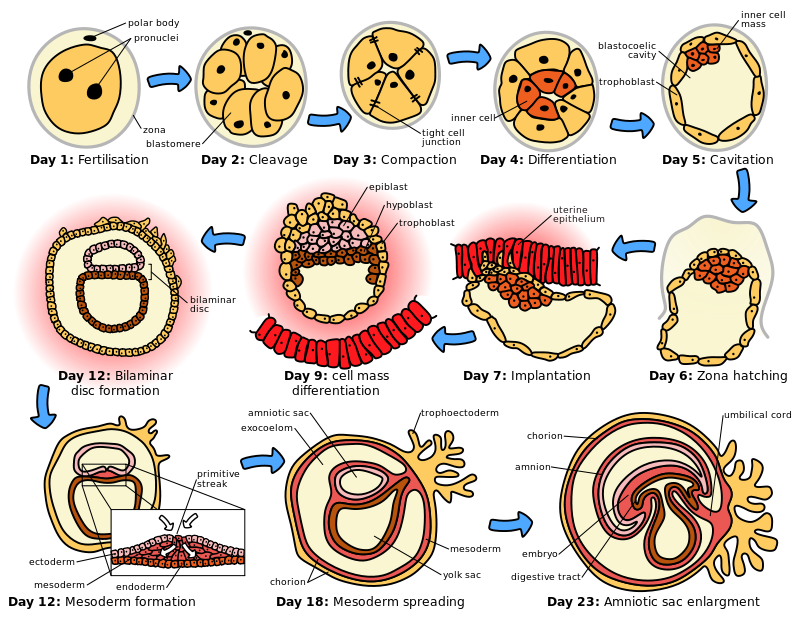
\includegraphics[width=15cm]{Chapter1/Fig/wiki_human_embryogenesis.png}
\caption[\textbf{Human Embryogenesis}]{\textbf{Human Embryogenesis}.\\
Placeholder adapted from wiki - stages of human embryogenesis}
\label{fig:embryogenesis}
\end{figure}

The next stage of early embrogenesis is gastrulation.
During gastrulation, the three germ layers (endoderm, mesoderm, ectoderm) form; the cell mass is now known as a gastrula.
A germ layer is a layer of cells that will go on to form one of our organizational tubes.
The first step of gastrulation is the formation of the primitive streak ($\sim$day 16).
This streak determines the midline of the body, and separates the left and right sides.
At this point, cells are moving down from the epiblast ending up between the original epiblast layer and the hypoblast.
The first layer to invaginate dives the deepest and ends up closest to the hypoblast - this is the endoderm.
The next layer forms the mesoderm, and the remaining epiblast cells that continue to border the amniotic cavity are the ectoderm.\\

The next stage is called neurulation.
Directly beneath the primitive streak the mesoderm (the middle germ layer) forms a thin rod of cells known as the notochord.
The notochord induces a change within the ectoderm above it, which is the formation of the neural plate dove into the mesoderm to form then neural tube, neurocrest cells.
That this the end of what is called "early embryogenesis".\\


Next, the germ layers start forming the various organs in a process called organogenesis.
Briefly, the endoderm forms the gastrointestial tract, from which upper tract the lungs, the liver, the pancreas form. 
The tube of course also form the oesophagus, the stomach, and the small and large intestine.
Second, the mesoderm forms some inner layers of the skin (endothelial), muscles (including the heart), bones and then also the kidneys and the bladder, ovaries and/or testis and blood cells.
Finally, the ectoderm, forms the outer layer of skin (epithelial) and sweat glands and hair and importantly our nervous system.
After 8 weeks since fertilization, we call the embryo a foetus, and fetal development starts.

% \subsubsection{Mechanisms of differentiation}

% Cues can be internal and external.

% Internal:

% zygote contains transcription factors (TFs) which will activate certain genes as well as their mRNA recursors.
% TFs are all clustered in one area of the zygote so as cells divide cells that were in the TF-rich region of the zygote will have many TFs while others will have barely any.
% This is known as "asymmetric segregation of cellular determinants".

% External: induction

% One group of cells can induce another group of cells to differentiate using signalling, which can be in the form of diffusion, direct cell-to-cell contact or gap junctions (connexon proteins) between cells.

% Examples: limbs, ears, eyes

% %********************************** % 1.2.2  **************************************
\subsection{Stem Cells}

% look up in humans
In mammals, roughly 50–150 cells make up the inner cell mass during the blastocyst stage of embryonic development, around days 5–14. 
These have stem cell\footnote{stem cells are characterised by their self-renewing abilities and the "potency" to differentiate into more specialised cells.} capability, meaning that they can eventually differentiate into all of the body's cell types (making them "pluripotent").

\begin{figure}[htbp]
\centering
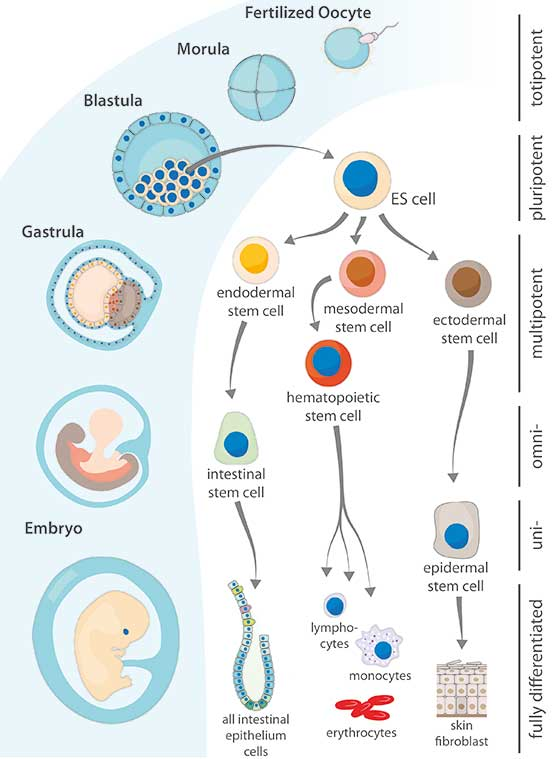
\includegraphics[width=13cm]{Chapter1/Fig/stem_cells.jpg}
\caption[\textbf{Stem Cells}]{\textbf{The potency tree of stem cells}.\\
Placeholder? from https://www.enzolifesciences.com/science-center/technotes/2019/august/stem-cells-from-embryonic-origin-to-induced-pluripotency-an-overview/}
\label{fig:stem_cells}
\end{figure}


% Inner cell mass stem cells are sometimes called "embryonic" stem (ES) cells to differentiate them from other types of stem cells found in the adult body, called somatic or adult stem cells.
% to maintain stem cell numbers:
% 1) obligate asymmetric replication i.e. each stem cell as it divides creates another stem cell and a differentiated cell
% 2) stochastic differentiation i.e. if one stem cells makes two differentiated cells instead, another will make two stem cells to balance it out
Only the zygote is considered to be truly "totipotent" as it is able to form not only cells of the body (derived from the epiblast) but extra-embryonic tissues as well (from the hypoblast), which are necessary for the formation of a living organism.
% Compared to ESCs, adult stem cells are less plastic, less potent.
Cells with stem-cell properties are still present in the adult body, and are called somatic or adult stem cells.
In general, they are less plastic (less potent) than inner mass cells.
In particular, some adult stem cells have the ability to differentiate into a whole suite of cell types, and are called "multipotent".
This is the case for example of hemapoietic stem cells, which give rise to all the cell types of the blood and the immune system.
Other stem cells are more specialised, like epidermal stem cells, which are only able to differentiate into fibroblasts.
These are called "unipotent" (Fig. \ref{fig:stem_cells}).\\

The existence of stem cells were first demonstrated by Canadian biologists Ernest McCulloch and James Till in the early 1960s.
Together with graduate student Andy Becker and senior scientist Lou Siminovitch the work was published in Nature in 1963 \cite{becker1963cytological}.


\subsubsection{Embryonic stem cells}

As mentioned before, inner mass cells are pluripotent.
\textit{In vivo}, they go on to differentiate into the three germ layers (during gastrulation) and then on to make up organs (during organogenesis).
In general, differentiation is thought to be a one-way street, meaning that more specialised cells cannot go backwards to stem cells naturally.
However, when they are isolated and cultured \textit{in vitro}, they can be kept in the stem-cell stage and are known as embryonic stem cells (ESCs).
In 1981, embryonic stem (ES) cells were first isolated and successfully cultured using mouse blastocysts by British biologists Martin Evans and Matthew Kaufman \cite{evans1981establishment, martin1981isolation}.
The first human embryonic stem cells (hESCs) were isolated in 1998 by American developmental biologist James Thomson.
Thomson and colleagues derived hESC lines by culturing human blastocysts in a cocktail of growth factors and supporting mouse feeder cells (Thomson et al., 1998) \cite{thomson1998embryonic}. 
These hESC lines were immediately heralded as foundational for cell replacement therapy and for modeling human diseases (Gearhart, 1998).
\cite{saha2009technical}

Note that to isolate ESCs one needs to destroy the embryo, which caused a big ethical debate.
In practice, a number of lines have been isolated and frozen and are available for research.
How many? Where? All healthy?
Up side: lines have been tested and looked at carefully and selected to have good properties etcetera

% \subsubsection{Stem Cell systems}
% Embryonic stem cells \& Organoid models
Emryonic stem cells have been used widely to improve our understanding of embryogenesis and development in general. 

They have been differentiated into x,y,z
ESC lines available have been carefully selected and are optimised for ..

ESCs can be grown in a 2D culture but also in 3D structures, to better mimick the formation of organs (organoids) or even entire (early) embryos (gastruloids).

Embryoid Bodies (EBs) - ESCs left to aggregate with the addition of some cytokines (Brickman and Serup 2016, Spangler et al 2018)

micropatterns: MPA vs MPP (anteriorly or posteriorly biased)
Morgani et al 2018

Gastruloid can break symmetry - form antero-posterior axis (van de Brink et al 2014, van den Brink 2020)

PGC: primordial germ cells

As far as 

% %********************************** % 1.2.3  **************************************
\subsection{Nuclear cloning of somatic cells}

Nuclear cloning, also referred to as nuclear transfer or nuclear transplantation, denotes the introduction of a nucleus from an adult donor cell into an enucleated oocyte to generate a cloned embryo \cite{hochedlinger2003nuclear}.
When transferred to the uterus of a female recipient, this embryo has the potential to grow into an infant that is a clone of the adult donor cell, a process termed “reproductive cloning.” 
However, when explanted in culture, this embryo can give rise to embryonic stem cells that have the potential to become any or almost any type of cell present in the adult body.\\

The word "clone" comes from the Greek word for XX, it was first applied in plants.

The first to perform nuclear cloning in animals was British developmental biologist Sir John Gurdon. 
During his PhD in the Zoology department at Oxford, Gurdon worked on nuclear transplantation in a frog species of the genus \textit{Xenopus}.
In 1958, he successfully cloned a frog using intact nuclei from the somatic cells of a \textit{Xenopus} tadpole (ref).
This critical study proved that eggs receiving transplanted nuclei from a more mature cell type could be differentiated, directly contradicting what was believed at the time (king and Briggs) \cite{king1955changes}. \\

The first cloned mammal was Dolly the sheep, born on July 5, 1996.
She was cloned by Keith Campbell, Ian Wilmut and colleagues at the Roslin Institute at the University of Ediburgh, Scotland, using the process of somatic-cell nuclear transfer (SCNT).
Dolly had three mums: one provided an unfertilised oocyte (cytoplasmic donor), another who provided the nucleus (from a mammary gland cell, nuclear donor) and finally a surrogate ewe who hosted the embryo until its birth.
% She was named after Dolly Parton.

after that many specifies were cloned including pigs, cats, dogs, horse, camels and even macaques.

Problematic Lulu and Nana?

% clones die early, most embryos die soon after implantation, those that live have abnormalities, die prematurely, become obese or develop tumours.
% The phenotype does to an extent depend on the type of donor cell used.
% Not their offspring though, so maybe epigenetic rather than genetic.
% Faulty epigenetic reprogramming.
% Cloning from embryonic stem cells is roughly 10 to 20 times as efficient as cloning from somatic cells (specific genes are already active).
% i.e. 1-3\% vs 10-30\%.

% Note: Prezygotic reprogramming includes the acquisition of genomic imprints — the expression of genes from either the paternal or maternal set of chromosomes — as well as the modification of most somatic genes during gametogenesis. Inactivation of the X chromosome and adjustment of the length of telomeres are examples of postzygotic reprogramming.

Somatic (differentiated) cells can be reprogrammed by transferring their nuclear contents into (enucleated) oocytes (Wilmut et al 1997) or by fusion with ES cells (Cowan et al 2005, Tada et al 2001).

In 2003, XX wrote a review on cloning, identifying cloned embryos explanted in culture as the only way to obtain 

That was indeed true until in 2006, Japanese stem cell researcher Shinya Yamanaka successfully managed to re-programme mouse fibroblasts into acquiring a stem-cell identity, generating the first induced pluripotent stem cells (iPSCs) \cite{takahashi2006induction}.

The next year, the labs of Yamanaka and Thomson successfully generated iPSCs from human somatic cells \cite{takahashi2006induction, }, surclassing nuclear transplantation as the first step toward effective regenerative medicine.\\

In 2012 Sir John B. Gurdon and Shinya Yamanaka were jointly awarded the Nobel Prize in Physiology or Medicine "for the discovery that mature cells can be reprogrammed to become pluripotent" (ref).    




% %****** Box on model organisms ******

% %\newpage

% \begin{Comment}
% \hspace{-2.5mm}\textbf{Box 2: Model organisms}\label{box2}\\
% % \small

% Model organisms are non-human species used to study biological phenomena:

% \begin{itemize}
%     \item Bacteria (\textit{Escherichia coli}, or \textit{E. coli})
%     \item Budding Yeast (\textit{Saccharomyces cerevisiae} or \textit{S. cerevisiae})
%     \item Thale cress (\textit{Arabidopsis Thaliana})
%     \item Fruit fly (\textit{Drosophila melanogaster})
%     \item Nematode worm (\textit{Caenorhabditis elegans} or \textit{C. elegans})
%     \item Western clawed frog (\textit{Xenopus tropicalis})
%     \item Zebrafish (\textit{Danio rerio})
%     \item Mouse (\textit{Mus musculus})

% \end{itemize}


% \end{Comment}

% %**************


% %********************************** % 1.2.1  **************************************
\subsection{Induced pluripotent stem cells}

% advantage of iPSCs over ESCs
Use of human embryos, however, faces ethical controversies that hinder the applications of human ES cells. In addition, it is difficult to generate patient- or disease-specific ES cells, which are required for their effective application \cite{yamanaka2007strategies}.

The induction of pluripotent stem cells from somatic cells was first demonstrated in mice in 2006.

In a paper published in Cell, Takahashi and Yamanaka first demonstrated induction of pluripotent stem cells from both embryonic or adult mouse fibroblasts by inducing four transcription factors, Oct3/4, Sox2, c-Myc and Klf4, under ES cell culture conditions
\cite{takahashi2006induction}.

They could show that iPSCs exhibited similar morphology, proliferation properties and doubling times compared to ESCs.

% They began with a set of 24 candidate genes that were i) known to play a role in the maintenance of pluripotency (such as Oct3/4 and Sox2, but also Nanog), ii) frequently up-regulated in tumours and that contribute to maintenance of ES cell phenotype and rapid proliferation (e.g. Stat3, c-myc) as well as iii) other genes specifically expressed in ES cells. 

% Genes were introduced into mouse embryonic fibroblasts (MEFs) from Fbx15 embryos by retroviral transduction (use the property of RNA viruses to insert a copy of its genome into the DNA of a host cell that it invades to introduce specific sequences into a cell?).

% Tried different combination and kept colonies exhibiting similar morphology, proliferation properties and doubling times.

A year later, the Yamanaka and Thomson labs published around the same time induction of pluripotent stem cells in human \cite{takahashi2007induction}.
Both derived human iPSCs from fibroblasts, but:

the Yamanaka paper from adult human dermal fibroblasts 
retroviral system and using the same 4 factors Oct3/4, Sox2, c-Myc and Klf4
% show embryoid bodies mediated as well as direct differentiation
% neural, cardiac cells

Thomson paper: lentiviral system
and different factors: Oct4, Sox2 and Nanog + Lin28 instead.

\subsubsection{Technical aspects of iPSC induction}

OSKM factors or Yamanaka factors
It has been shown that the first transcriptional wave is mostly mediated by c-Myc and occurs in all cells whereas the second wave is more restricted to reprogrammable cells and involves a gradual increase in the expression of Oct4 and Sox2 targets, leading to the activation of other pluripotency genes that aid in the activation of the pluripotency network. Klf4 seems to support both phases by repressing somatic genes during the first phase and facilitating the expression of pluripotency genes in the second phase \cite{buganim2013mechanisms}.\\

Varying factors:
Factors used (Oct3/4, Sox2, c-Myc, Klf4)
Factor induction system (\cite{narsinh2011comparison} Narsinh, Plews and Wu, 2011)
\begin{itemize}
    \item viral transduction
    \item DNA-based induction + plasmid transfection
    \item mRNA transfection
    \item recombinant proteins and protein tranduction
\end{itemize}
Cell types of origin: dermal skin fibroblasts \cite{takahashi2007induction},
adipocytes (Sugii et al 2010), nucleated blood cells (Loh et al 2009),
and dental pulo (Yan et al 2010). From \cite{} (Zanella, Lyon ans Sheikh 2014)

keratinocytes, peripheral blood cells, epithelial cells


\subsubsection{Challenges in the use of iPSCs}
Low efficiency has been recorded in the generation of iPSCs.
On average, XX\% of the starting cells effectively exhibit pluripotency and can be used for further studies

Additionally, mutations can be accumulated during the reprogramming process.

Tumorigenicity has been observed, and only partially solved by removing oncogene c-myc.

Finally, incomplete reprogramming has been observed, with cells maintaining an "epigenetic memory".

The epigenetic signature of the somatic cell must be erased during the conversion in order to adopt a stem cell-like epigenome. These changes include chromatin reorganization, DNA demethylation of promoter regions of pluripotency genes like Nanog, Sox2 and Oct4, reactivation of the somatically silenced X chromosome, and genome-wide resetting of histone posttranslational modifications11,30–32.
from Buganim ert al, 2013 \cite{buganim2013mechanisms}

iPSCs are heterogeneous due to random X inactivation in cell lines derived from female indivuduals.



low efficiency
genomic insertions
tumorigenicity 
(mutations accumulated suring the reprogramming process)
incomplete reprogramming (epigenetic memory)
iPSCs are heterogeneous (random X inactivation)
\cite{halevy2014comparing} (Halevy and Urbach 2014)

\cite{park2008reprogramming}

Reprogramming of human somatic cells uses readily accessible tissue, such as skin or blood, to generate embryonic-like induced pluripotent stem cells (iPSCs). \cite{saha2009technical}



% %********************************** % 1.2.1  **************************************
\subsection{Clinical applications of human stem cells}

"The promise of induced pluripotent stem cells in research and therapy" \cite{robinton2012promise}

first human embryonic stem cells (ESCs) based model (a model for Lesch-Nyhan syndrome by targeting of the HPRT gene in human ESCs)\cite{urbach2004modeling}
\cite{halevy2014comparing}

other models were further used to obtain novel mechanistic or physiological insights regarding the disorders. One example is a model for Amyotrophic Lateral Sclerosis (ALS) by Kiskinis et al \cite{kiskinis2014pathways} \\


\textbf{mouse iPSCs} (paragraph from Saha and Jaenish 2009 \cite{saha2009technical}):
Recent work with rodents has tested the developmental potential of iPSCs and their potential for the treatment of diseases. Differentiation of mouse iPSCs can be directed in vitro into cardiovascular (Kuzmenkin et al., 2009; Narazaki et al., 2008; Schenke-Layland et al., 2008), hematopoietic (Hanna et al., 2007; Schenke-Layland et al., 2008; Xu et al., 2009), neural (Wernig et al., 2008), and hepatic progenitor cells (Cantz et al., 2008), and recently, mouse iPSCs passed the most stringent test of pluripotency by generating full-term adult mice in tetraploid complementation assays (Boland et al., 2009; Kang et al., 2009; Zhao et al., 2009). Further, mouse iPSCs obtained from adult fibroblasts can be used to restore physiological function of diseased tissues in vivo, as demonstrated by using iPSC-derived hematopoietic cells in a humanized mouse model of sickle cell anemia (Hanna et al., 2007). Also, endothelial/endothelial progenitor cells derived from mouse iPSCs injected directly into the liver of irradiated hemophilia A mice extended their survival for more than 3 months and rescued depleted Plasma FVIII levels (Xu et al., 2009). Finally, functional dopamine neurons could be generated from reprogrammed mouse fibroblasts, and transplantation of these neurons, like mESC-derived neurons, could restore dopamine function when grafted into Parkinsonian rats (Wernig et al., 2008). These studies establish that iPSCs have vast potential to generate a variety of functional cell types and can be used to modify the course of disease in rodents.\\

\textbf{human iPSCs} (paragraph from Saha and Jaenish 2009 \cite{saha2009technical}):
Differentiation of hiPSCs into several cell types has already been achieved: neural progenitors (Chambers et al., 2009), motor neurons (Dimos et al., 2008; Ebert et al., 2009), dopaminergic neurons (Soldner et al., 2009), retinal cells (Osakada et al., 2009), hepatocytes (Sullivan et al., 2009), blood cells (Choi et al., 2009; Ye et al., 2009), adipocytes (Taura et al., 2009), endothelial cells (Choi et al., 2009; Sullivan et al., 2009), and fibroblasts (Hockemeyer et al., 2008; Maherali et al., 2008). 





feeder: inactivated embryonic fibroblasts

feeder-free is cheaper quicker more ethical

teratoma assay to assess pluripotency.
A teratoma is a non-malignant tumour that contains a mixture of cells from all three germ layers.
iPSCs or hESCs can be injected into an immuno-suppressed mouse and then we can wait until the mouse develops a teratoma and perform histological analysis of it to check that all layers (ecto, meso and endodermal cells) are present.


The promise of using pluripotent stem cells (PSCs) for regenerative medicine dates back to 1998 when James Thomson \cite{thomson1998embryonic} first derived human embryonic stem cells (hESCs) from the inner cell mass of developing embryos \cite{kimbrel2015current}.
Not only do PSCs have the ability to self-renew indefinitely, but in theory they can also be differentiated into any cell type in the body, thus providing functional replacement or trophic support to worn-out or dysfunctional cells and tissues in a range of diseases. \\

During the 2000s, funding restrictions and ethical concerns provided the impetus to find alternative approaches to generating stem cells with the same degree of pluripotency as hESCs. 
Induced pluripotent stem cell (iPSC) technology quickly became the leading alternative to hESCs \cite{takahashi2006induction, takahashi2007induction, yu2007induced}
The generation of iPSCs involves the reprogramming of differentiated somatic cells into a pluripotent state by the introduction of a cocktail of factors to 'reset' the transcriptional programme of the cell back to an embryonic state. 
In 2012, Shinya Yamanaka and Sir John Gurdon11 were awarded a Nobel Prize for their combined efforts in discovering that “mature cells can be reprogrammed to become pluripotent”. 

\subsubsection{tissues and diseases}

\textbf{Nervous system.}
Disease-specific iPSC-derived neurons are also being used as in vitro models to elucidate the cellular and molecular pathogenesis of Parkinson disease83,84,85,86,87, Alzheimer disease88,89, ALS90,91,92,93, spinal muscular atrophy94,95 and others.


\begin{itemize}
    \item ESCs (embryonic stem cells)
    \item TSPSCs (tissue-specific progenitor stem cells)
    \item MSCs (mesenchymal stem cells)
    \item UCSCs (umbilical cord stem cells)
    \item BMSCs (bone marrow stem cells)
    \item iPSCs (induced pluripotent stem cells)
\end{itemize}

list from \cite{mahla2016stem}


add timeline from (Current status of pluripotent stem cells: moving the first therapies to the clinic,  figure 2)

\cite{kimbrel2015current}

aurologous vs allogenic (ESCs are genetically different from receiver) transplant

\subsubsection{ESCs vs iPSCs}

genetic variation
genome editing in ESCs not very efficient
much easier to derive iPSCs with a given genetic background

obvious ethical concerns and limitations (e.g. some countries might ban studies using ESCs altogether)

most famous clinical application of stem cells is in laeukemia patients
cells grow uncontrollably and prevent hematopoietic stem cells to proliferate so you can kill them with chemo/radio therapy and then transplant hematopoietic SCs back in (stem cell therapy?)


% %********************************** % 1.2.1  **************************************
% \subsection{iPSC consortia}

\subsection{Applications of human iPSCs in genetics}

In order to obtain an ES cell one must destroy the embryo, raising ethical concerns that caused the generation of ESCs reduced substantially or even made illegal in some countries.

In contrast, iPSCs can be derived from easily accessible tissues such as blood or skin, bypassing all such concerns.

Because they are very easy to derive, they can be generated for specific patients, or people with genetic disorders we might want to study.

Down the line, iPSC technology opens the way to regenerative medicine where tissues can be re-generated with one's own cells thus avoiding the risk of immune rejection (when the body rejects a donor's allogenic organ as a foreign object).

In addition to genetic disorders and tissue regeneration, the iPSC technology can be applicable to basic science research of human development and disease modeling.

Human iPSCs have already been differentiated into: 
differentiated to cardiomyocytes, neurons, endoderm, retina

neural stem cell, cortical neuron (Shi et al 2012), dopaminergic neuron (Ma et al 2011), motor neuron (Karumbayaram et al 2009), astrocyte (Shaltouki et al 2013), oligodendrocyte (Douvaras et al 2014)
cardiomyocyte (Burridge, et al 2014), skeletal muscle (Maffioletti et al 2015), vascular endothelial/smooth muscle (Patsch et al 2015)
hepatocyte (Si-Tayeb et al 2009), pancreatic beta cell (Zhang et al 2009), lung (Huang et al 2013)\\



\textbf{HipSci}
The \gls{hipsci} is the largest of such consortia, and we will use data from \gls{hipsci} \cite{kilpinen2017common} throughout this thesis.

System: sendai vectors expressing  
Factors: human (h)OCT3/4, hSOX2, hKLF4 and hMYC
Cell of origin: primary fibroblasts
Medium:
Pluripotency score: novelty score + pluritest \cite{muller2011bioinformatic}
Samples:

Transduced cells were culture on an irradiated mouse embryonic fibroblast (MEF-CF1) feeder
picked between day30 and 40 and cultured in iPS cell medium until ready to passage (define). 
Cells passaged evert 5-7 days until established (usually at passage 5 or 6)
then lines expanded for banking and characterization
now transferred to feeder-free culture\\

\textbf{other iPSC consortia and large studies}

iPSCORE \cite{panopoulos2017ipscore}, GENESiPS \cite{carcamo2017analysis}, PHLiPS \cite{pashos2017large}, Banovich \textit{et al} \cite{banovich2018impact}

\subsubsection{eQTL mapping using iPSCs and iPSC-derived cells}

In 2017, the \gls{hipsci} consortium published their flagship paper, where they assessed iPSC lines through various assays, and mapped eQTL in XX cell lines from YY unique donors
\cite{kilpinen2017common}.

At around the same time, another map of iPSC eQTL was published in XX \cite{deboever2017large}.

Most recently, a meta-study was published as the result of an effort to combine iPSC resources into the i2QTL consortium  
\cite{bonder2019systematic}.\\

eQTL have also been mapped in iPSC-derived cell types.

These include iPSC derived XX neurons \cite{schwartzentruber2018molecular}, and ...

\newpage

\section{Thesis outline}

The overall aim of this thesis is to provide suitable methods to perform eQTL mapping at single cell resolution and to explore the effects of common genetic variants on single cell expression across a range of human iPSC-derived cell types using data from the HipSci project.\\

Specifically, in Chapter 2, I give an overview of current LMMs for genetic analyses, covering their use for association and interaction testing, focusing on their application in eQTL mapping.\\

In Chapter 3, I describe best practice approaches to perform eQTL mapping using scRNAseq profiles and demonstrate these nethods on matched bulk and single cell expression of around 100 human iPSC lines as well as on simulated data.  \\

In Chapter 4, I present a dataset of almost 40,000 cells from 125 human iPSC lines differentiating to definitive endoderm, and demonstrate different approaches to eQTL mapping using scRNA-seq data, identifying genetic variants that affect gene expression dynamically along differentiation. \\

In Chapter 5, I present a dataset of over 1 Million cells from 215 human iPSC lines to midbrain neurons.
We identify thousands of eQTL across a number of cell types and upon external stimulation and identify hundreds of colocalization events with variants known to be associated with neurological traits and disease.
Additionally, we investigate sources of variation in the capacity of individual cell lines to differentiate toward neurons.\\

In Chapter 6, I present a novel method to jointly test for context-specific eQTL across multiple cell types and states defined at single cell resolution. \\

Finally, in Chapter 7 I conclude and discuss future directions.